% !TeX program = pdflatex
% 基于提供的 Medical Physics 2021 模板。使用 pdfLaTeX 编译两次。
% 内容来自 manuscript-20261029.docx；修改正文后重新编译。
\documentclass[12pt,twoside,letterpaper]{article}
\usepackage[T1]{fontenc}
\usepackage[utf8]{inputenc}
\usepackage{lmodern}
\usepackage{amsmath,amssymb}            % 数学公式
\usepackage{graphicx}                   % 图片
\usepackage{placeins}                   % 在必要边界清理待排图表
\usepackage{float}                      % 图表保留在对应正文位置
\usepackage{booktabs,array,tabularx}                   % 三线表
\usepackage[super,sort&compress,comma]{natbib} % 上标数字引用，连续编号合并为范围
\usepackage{setspace}                   % 行距
\usepackage[mathlines]{lineno}          % 连续行号
\modulolinenumbers[5]                  % 每 5 行显示一次行号
\usepackage{fancyhdr}                   % 页眉与页脚
\usepackage[hidelinks]{hyperref}        % 可点击的引用和链接
\graphicspath{{figures/}}               % 图片放在 figures 文件夹

% 页面尺寸与章节编号，一般不需要修改。
\setlength{\textwidth}{16.5cm}
\setlength{\textheight}{22.6cm}
\setlength{\oddsidemargin}{-1mm}
\setlength{\evensidemargin}{-2mm}
\setlength{\topmargin}{-1cm}
\setlength{\headheight}{15pt}
\setlength{\headwidth}{\textwidth}
\setlength{\parindent}{0pt}             % 段落首行不缩进
\setlength{\parskip}{1.3ex}
\renewcommand{\thesection}{\Roman{section}.}
\renewcommand{\thesubsection}{\thesection\Alph{subsection}.}
\renewcommand{\thesubsubsection}{\thesubsection\arabic{subsubsection}.}
\makeatletter
\renewcommand\@biblabel[1]{$^{#1}$}
\makeatother
\setlength{\bibhang}{0em}


\setlength{\emergencystretch}{3em}

% 所有页面右上角显示页码，页眉为细横线，页脚留空且无线条。
\pagestyle{fancy}
\fancyhf{}
\fancyhead[R]{\thepage}
\renewcommand{\headrulewidth}{0.4pt}
\renewcommand{\footrulewidth}{0pt}
\fancypagestyle{plain}{%
  \fancyhf{}
  \fancyhead[R]{\thepage}
  \renewcommand{\headrulewidth}{0.4pt}
  \renewcommand{\footrulewidth}{0pt}
}


% 全文单栏；图表自动适配页面宽度。

% Allow nearby text and floats to share a page; avoid sparse float-only pages.
\renewcommand{\topfraction}{0.95}
\renewcommand{\bottomfraction}{0.90}
\renewcommand{\textfraction}{0.05}
\renewcommand{\floatpagefraction}{0.98}
\setcounter{topnumber}{3}
\setcounter{bottomnumber}{3}
\setcounter{totalnumber}{6}
\setlength{\textfloatsep}{12pt plus 2pt minus 2pt}
\setlength{\intextsep}{12pt plus 2pt minus 2pt}

\begin{document}

\raggedbottom

\begin{center}

{\Large\bfseries Integrated Optimization of Catheter Number and Spatial Configuration for Individualized Template-Guided High-Dose-Rate Interstitial Brachytherapy\par}

\vspace{6mm}

Qinglong~Yao, B.S.\textsuperscript{1}, Zhuo~Xiao, M.S.\textsuperscript{1}, Fugen~Zhou, Ph.D.\textsuperscript{1}, Junjie~Wang, M.D., Ph.D.\textsuperscript{2}, Qiuwen~Wu, Ph.D.\textsuperscript{3}, Haitao~Sun, M.S.\textsuperscript{2}, Ping~Jiang, M.D.\textsuperscript{2,*}, Bo~Liu, Ph.D.\textsuperscript{1,*}\par

\vspace{4mm}

{\small

\emph{\textsuperscript{1} Image Processing Center, Beihang University, Beijing 100191, People's Republic of China}\par

\emph{\textsuperscript{2}} \emph{Department of Radiation Oncology, Peking University Third Hospital, Beijing 100191, People's Republic of China}\par

\textsuperscript{\emph{3}} \emph{Department of Radiation Oncology, Duke University Medical Center, Durham, North Carolina 27708, USA}\par

}

\end{center}

\textbf{Corresponding Authors}\par

\begingroup\small\setlength{\parskip}{0.4ex}

Bo Liu, Ph.D.\par

Image Processing Center\par

Beihang University\par

Beijing, 100191\par

P.R. China\par

Email: \href{mailto:bo.liu@buaa.edu.cn}{bo.liu@buaa.edu.cn}\par

\smallskip

Ping Jiang, M.D.\par

Department of Radiation Oncology\par

Peking University Third Hospital\par

Beijing, 100191\par

P.R. China\par

Email: \href{mailto:Jiangping@bjmu.edu.cn}{Jiangping@bjmu.edu.cn}\par

\smallskip

\endgroup

\clearpage

\begingroup\setlength{\parskip}{0.5ex}

\begin{abstract}

\noindent \textbf{Background}: Individualized template-guided high-dose-rate interstitial brachytherapy (HDR-ISBT) permits flexible catheter placement, but catheter number and configuration remain difficult to determine automatically.\par

\noindent \textbf{Purpose}: To develop and retrospectively evaluate an automated planning approach integrating catheter number determination with spatial configuration and dwell-time optimization for individualized template-guided HDR-ISBT.\par

\noindent \textbf{Methods}: We retrospectively replanned 94 fractions from 26 patients with locally recurrent cervical cancer. Feasible straight-catheter trajectories were generated, and an initial catheter pool was constructed through dose-guided selection and random supplementation. Group-sparsity optimization using the fast iterative shrinkage-thresholding algorithm (FISTA), followed by sequential pruning, determined catheter number without prespecifying the final count. Simulated annealing (SA)-based catheter exchange and local geometric fine-tuning subsequently optimized spatial configuration at that count, with dwell-time reoptimization. Automated plans were compared with clinical plans and across optimization stages. Ablation analyses assessed the azimuthal constraint, initial-pool construction, and sparsity weighting. Dosimetric metrics were evaluated after normalization to a high-risk clinical target volume (HR-CTV) D\textsubscript{90} of 600 cGy. Statistical inference used patient-level two-sided Wilcoxon signed-rank tests with a significance threshold of \emph{P} < 0.01.\par

\noindent \textbf{Results}: Compared with clinical plans, automated plans reduced the median catheter count from six to four (\emph{P} < 0.001), with fewer catheters in 78 of 94 plans. HR-CTV D\textsubscript{95} showed a median paired decrease of 5.7 cGy (\emph{P} = 0.002), whereas V\textsubscript{150} and V\textsubscript{200} did not differ significantly. Colon D\textsubscript{2cc} and urethral D\textsubscript{0.1cc} showed median paired decreases of 3.3 cGy (\emph{P} = 0.008) and 15.7 cGy (\emph{P} < 0.001), respectively; other organ-at-risk dose differences were not significant. Stage-wise analysis showed that the Group-sparsity optimization yielded a median of five catheters versus six clinically (\emph{P} = 0.016), with a small D\textsubscript{95} decrease and lower urethral D\textsubscript{0.1cc}. Pruning further reduced the median count to four but decreased D\textsubscript{95} and increased V\textsubscript{150}, V\textsubscript{200}, and organ-at-risk doses. Subsequent SA-based spatial configuration optimization improved D\textsubscript{95} and reduced V\textsubscript{150}, V\textsubscript{200}, and several organ-at-risk doses at the retained count. Ablation analyses showed that differential weighting yielded fewer catheters than uniform weighting within the same dose-guided pool, accompanied by higher V\textsubscript{200} and colon D\textsubscript{2cc}. Under uniform weighting, dose-guided and random pools showed no significant differences in catheter count or dosimetry. Median total optimization time was 510.6 s.\par

\noindent \textbf{Conclusions}: The integrated automated approach reduced catheter use with a small HR-CTV D\textsubscript{95} trade-off, while subsequent SA improved dosimetric performance at the retained count. Prospective pre-implantation planning and physical validation are required before clinical implementation.\par

\end{abstract}

{\small\noindent\textbf{Keywords:} High-dose-rate interstitial brachytherapy; individualized template; automated treatment planning; catheter configuration optimization; group sparsity; simulated annealing\par}

\endgroup

\clearpage

\setstretch{1.5}

\linenumbers

\section{Introduction}\label{sec:1}

High-dose-rate interstitial brachytherapy (HDR-ISBT) is an important salvage treatment option for patients with locally recurrent cervical cancer after pelvic irradiation.\cite{ref1,ref2,ref3,ref4} In HDR-ISBT, achieving the intended dose distribution requires appropriate planning of catheter configuration (including catheter number, positions, and directions) and dwell times, together with accurate reproduction of the planned catheter spatial configuration during implantation.\cite{ref5,ref6,ref7,ref8,ref9,ref10,ref11,ref12,ref13} In recent years, medical imaging and three-dimensional (3D) printing have supported the development of individualized templates and applicators for gynecological brachytherapy.\cite{ref14,ref15,ref16,ref17,ref18,ref19,ref20,ref21,ref22,ref23,ref24} Among these, 3D-printed individualized templates (3D-PITs) guide catheter insertion along predefined trajectories and support accurate implementation of patient-specific catheter configurations. However, template guidance does not directly determine an appropriate catheter configuration; catheter number still depends largely on planner experience, making systematic evaluation of the dosimetric performance achievable with different catheter counts difficult and potentially resulting in unnecessary catheter use.\cite{ref9,ref10,ref11,ref12,ref25,ref26} Furthermore, assessing three-dimensional collisions between nonparallel catheters complicates manual configuration design and may lead planners to restrict insertion directions, potentially limiting the geometric flexibility afforded by individualized templates.\cite{ref25} Therefore, an integrated automated planning framework for 3D-PIT-guided HDR-ISBT is needed to determine catheter number and optimize catheter spatial configuration and dwell times under anatomical and geometric constraints, with the aim of reducing unnecessary catheter use while balancing target coverage and organ-at-risk sparing.

Previous studies have explored various aspects of automated HDR brachytherapy planning. One line of research has developed inverse planning models\cite{ref27,ref28,ref29,ref30,ref31,ref32,ref33,ref34,ref35,ref36,ref37} to automate dwell-time optimization with catheter number, spatial configuration, and dwell positions specified in advance.\cite{ref38,ref39,ref40,ref41,ref42,ref43,ref44,ref45,ref46} Other studies have extended optimization to catheter spatial configuration,\cite{ref26,ref47,ref48,ref49,ref50,ref51,ref52,ref53,ref54} including methods that jointly optimize straight-catheter positions or directions and dwell times at a prespecified catheter count,\cite{ref55,ref56} as well as template-specific automated planning frameworks that integrate catheter design with dose optimization.\cite{ref25,ref57} Learning-based multi-atlas registration has also been used to predict catheter configurations before dwell-time optimization.\cite{ref58} Trajectory design has also been extended to curved paths,\cite{ref59,ref60,ref61,ref62,ref63,ref64} for example, by generating and selecting mechanically feasible curved needle channels within patient-specific applicators before dose optimization.\cite{ref65,ref66} Alongside catheter spatial configuration, determining catheter number is another key planning decision.\cite{ref67} Geometric-coverage-based greedy selection has also been used to generate catheter configurations without prespecifying catheter number, followed by dwell-time optimization and dosimetric plan selection.\cite{ref26} Other approaches optimize catheter spatial configurations and dose plans at multiple prespecified catheter counts and compare the resulting plans to assess the feasibility and dosimetric consequences of catheter reduction, providing a basis for selecting the final count.\cite{ref25,ref48,ref55,ref68} Catheter selection has also been incorporated into inverse planning through compressed sensing-inspired greedy methods\cite{ref69} or group-sparsity-based optimization.\cite{ref70,ref71} In the latter, penalties applied to catheter-specific dwell-time vectors promote the deactivation of individual catheters, allowing the retained catheters and their number to be determined jointly with dwell times. The fast iterative shrinkage-thresholding algorithm (FISTA)\cite{ref72} has been used to solve such group-sparsity optimization problems,\cite{ref70,ref71} and sparse catheter selection has also been combined with multicriteria dose optimization to generate candidate plans with different catheter numbers, spatial configurations, and dosimetric trade-offs.\cite{ref73}

These studies provide a methodological foundation for automated catheter planning. For 3D-PIT-guided HDR-ISBT, further investigation is needed into how template-constrained catheter generation and selection can be linked to adaptive catheter number determination and subsequent spatial configuration and dwell-time optimization. Fixing the catheter configuration or number in advance constrains optimization to the predefined dwell positions or catheter count, respectively.\cite{ref25,ref27,ref32,ref55} For approaches that support decision-making through candidate plans with different catheter counts, clinicians must still weigh catheter use against dosimetric quality to select the final count,\cite{ref74} which may entail additional time for manual evaluation and decision-making. Group-sparsity-based catheter selection can adaptively determine the retained catheters and their number.\cite{ref70,ref73} However, if their spatial configuration is not subsequently adjusted, further dose optimization is limited to dwell-time adjustments at the existing dwell positions, potentially restricting the ability to balance target coverage, high-dose volume control, and organ-at-risk sparing.\cite{ref70,ref71} Therefore, further optimization of catheter spatial configuration at the determined catheter count is warranted to provide additional degrees of freedom for improving the dose distribution.\cite{ref50,ref55,ref68}

We developed and retrospectively evaluated an integrated automated planning framework for straight-catheter HDR-ISBT in patients with locally recurrent cervical cancer, based on a 3D-PIT-guided ISBT protocol.\cite{ref20,ref21} The combined 3D-PIT comprises transvaginal and transperineal templates and allows catheter trajectories to be designed independently. The transperineal template can be customized to the patient's anatomy, with catheters guided through the transvaginal template into the target volume, as shown in Figure~\ref{fig:1}. Given patient anatomical contours, template geometry, and dosimetric objectives, the framework automatically generates candidate catheter trajectories incorporating an azimuthal constraint and constructs an initial catheter pool for optimization through dose-guided selection and random supplementation. Group-sparsity optimization and sequential pruning then determine the retained catheters and their number without prespecifying the final catheter count. Subsequently, catheter exchange and local geometric fine-tuning further optimize the spatial configuration while maintaining the determined count, with dwell times reoptimized during configuration updates. We compared automated plans with clinical plans for 94 fractions in 26 patients to evaluate catheter use, target coverage, and organ-at-risk sparing. Computational efficiency was also assessed, and stage-wise and ablation analyses were conducted to examine the roles of key planning components.

\FloatBarrier
\begin{figure}[H]
\centering
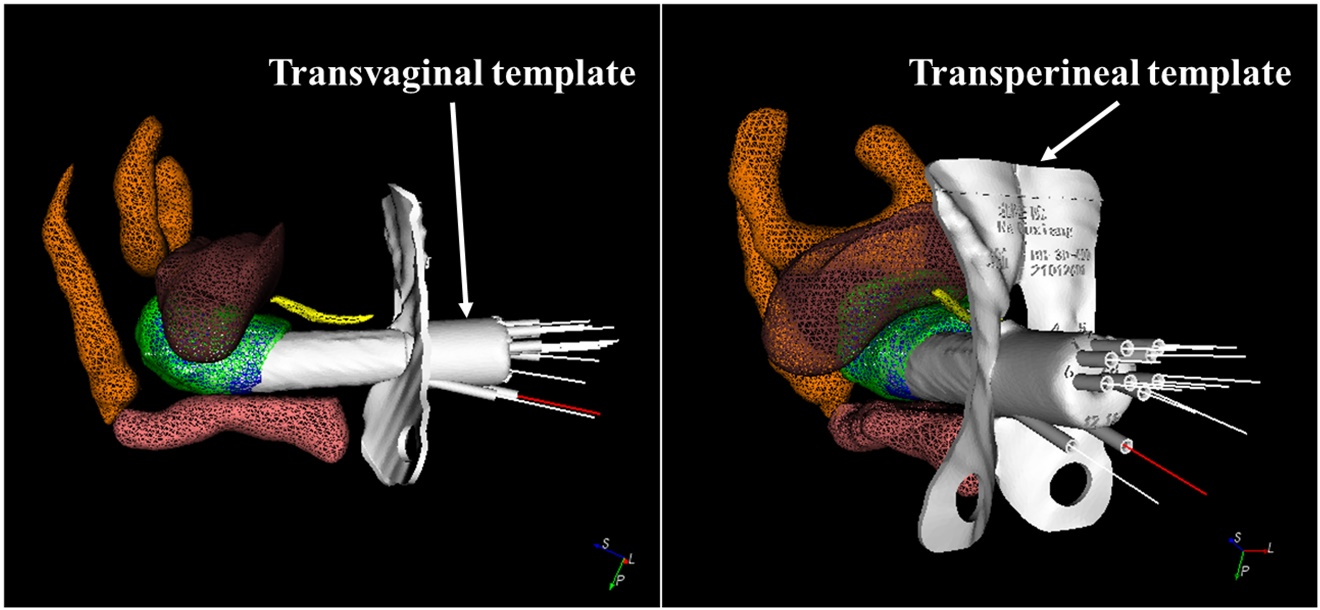
\includegraphics[width=0.92\linewidth,height=0.78\textheight,keepaspectratio]{figure1.jpg}
\caption{Three-dimensional visualization of the combined 3D-printed individualized template (3D-PIT), catheter trajectories, and patient anatomy from two viewing angles. The transvaginal and transperineal components are indicated in the left and right panels, respectively. White and red lines represent catheter trajectories, with the red line indicating the trajectory currently selected for viewing.}\label{fig:1}
\end{figure}

\section{Materials and Methods}\label{sec:2}

\subsection{Automated Catheter Planning Framework}\label{sec:2-1}

The proposed framework integrates catheter generation, catheter number determination, and spatial configuration and dwell-time optimization for 3D-PIT-guided HDR-ISBT using straight catheters. Given patient anatomical contours, template geometry, and dosimetric objectives, planning proceeds through three sequential stages, as illustrated in Figure~\ref{fig:2}.

\begin{enumerate}
\item Candidate trajectory generation and initial-pool construction. Candidate trajectories satisfying anatomical and geometric constraints are generated. Dose-guided selection and random supplementation then construct a geometrically compatible initial catheter pool for subsequent group-sparsity-based catheter selection and dwell-time optimization.
\item Adaptive catheter number determination. Group-sparsity optimization and sequential pruning select the retained catheters and determine their number without prespecifying the final catheter count. Dwell-time reoptimization is used to assess target-coverage feasibility during catheter reduction.
\item Catheter spatial configuration optimization. At the determined catheter count, catheter exchange and local geometric fine-tuning adjust the spatial distribution of available dwell positions. Dwell times are reoptimized to adapt the dose distribution to each updated configuration.
\end{enumerate}

\FloatBarrier
\begin{figure}[H]
\centering
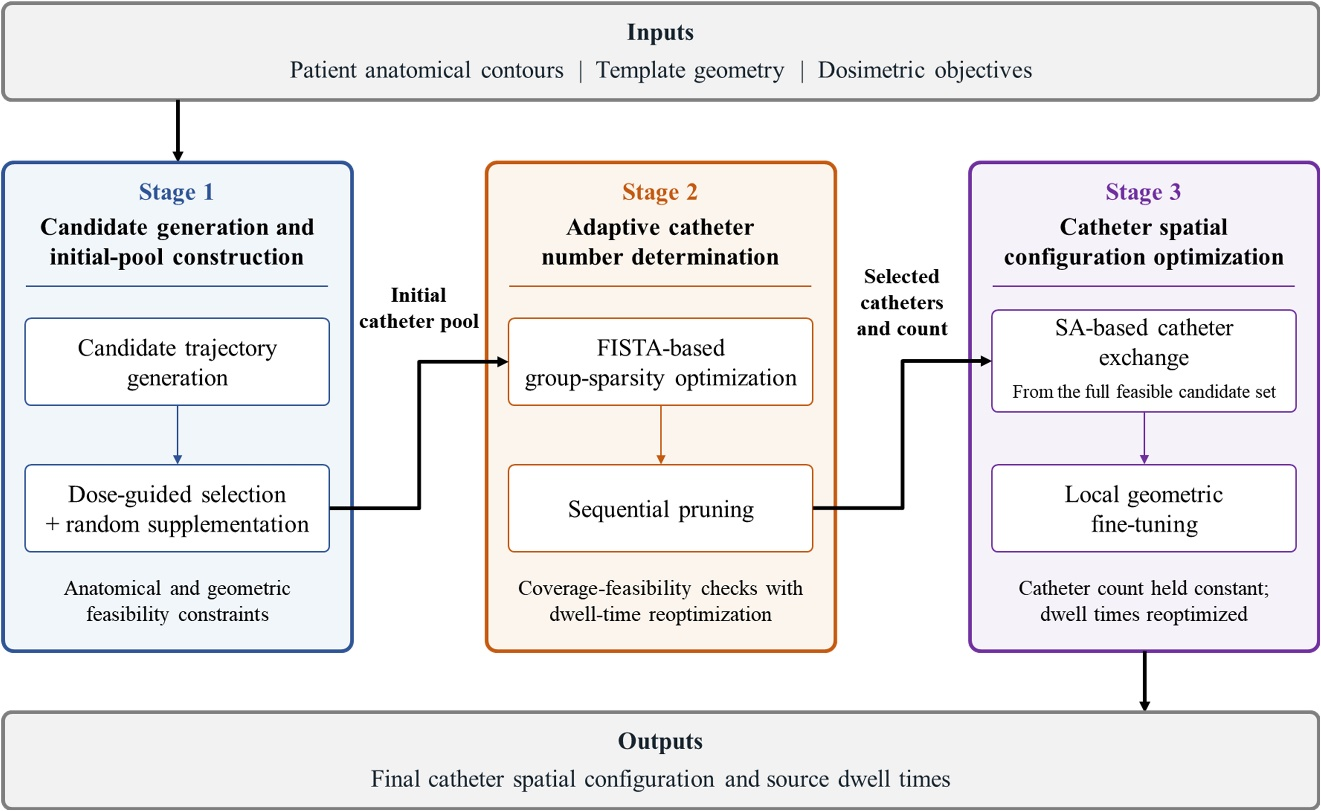
\includegraphics[width=0.92\linewidth,height=0.78\textheight,keepaspectratio]{figure2.jpg}
\caption{Overview of the integrated automated planning workflow for 3D-PIT-guided HDR-ISBT. FISTA, fast iterative shrinkage-thresholding algorithm; SA, simulated annealing.}\label{fig:2}
\end{figure}

\subsubsection{Candidate Trajectory Generation and Initial Pool Construction}\label{sec:2-1-1}

As illustrated in Figure~\ref{fig:3}(A), straight candidate trajectories were generated by connecting points sampled from anatomically feasible entry and target regions on their respective sampling planes, following the sampling approach of Yao et al.\cite{ref25} Each trajectory was truncated on the target side at the surface of the high-risk clinical target volume (HR-CTV). A trajectory was retained if it intersected the boundaries of both the HR-CTV and individualized template at least twice, traversed at least 10 mm within the HR-CTV and 50 mm within the template, and avoided contoured organs at risk (OARs) before entering the HR-CTV.

\FloatBarrier
\begin{figure}[H]
\centering
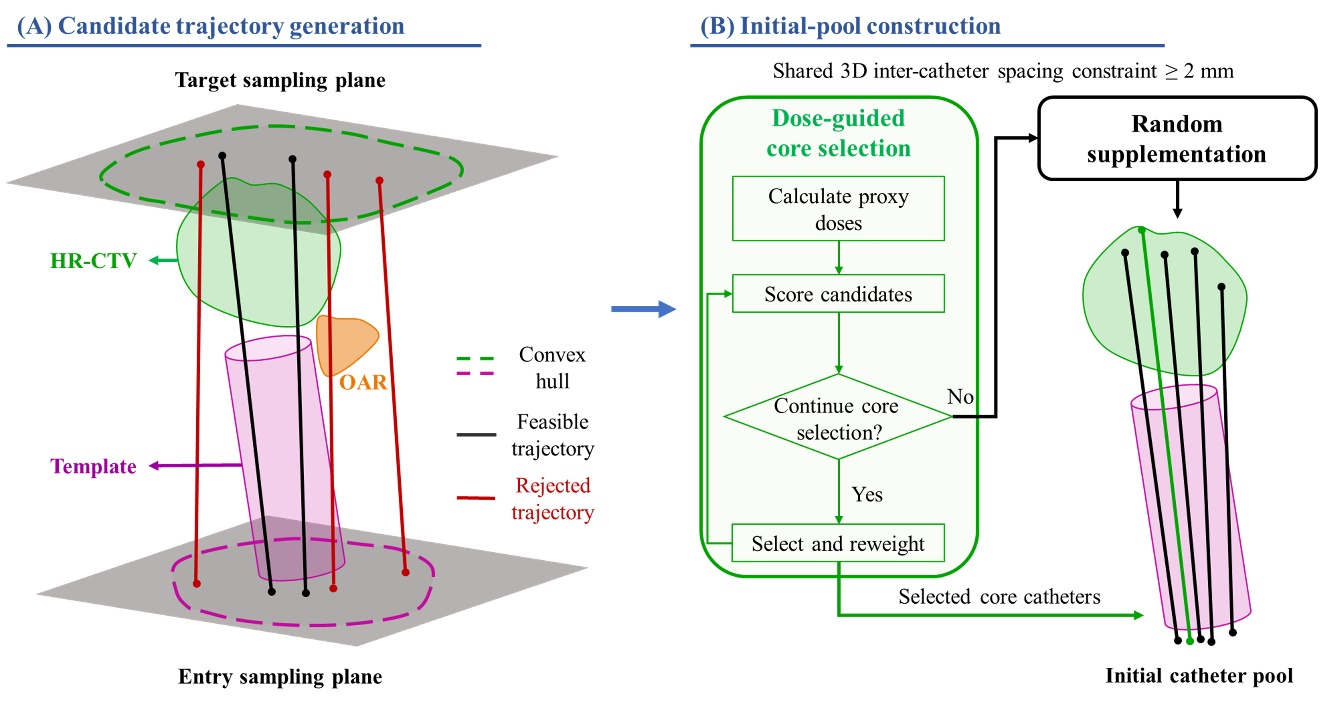
\includegraphics[width=0.92\linewidth,height=0.78\textheight,keepaspectratio]{figure3.jpg}
\caption{Candidate trajectory generation and initial-pool construction. (A) Generation and feasibility screening of candidate trajectories. (B) Initial-pool construction using dose-guided core selection and random supplementation. Green and black trajectories in (B) represent core and randomly supplemented catheters, respectively.}\label{fig:3}
\end{figure}

To discourage pronounced catheter crossings, an entry--target azimuthal consistency constraint was introduced. This constraint limits the difference between the azimuthal angles of the vectors from the respective sampling-region centers to the sampled entry and target points. The entry and target azimuthal angles were calculated as $\theta_{e} = \operatorname{atan2}\left( y_{e} - {\overline{y}}_{e},\ x_{e} - {\overline{x}}_{e} \right)$ and $\theta_{t} = \operatorname{atan2}\left( y_{t} - {\overline{y}}_{t},\ x_{t} - {\overline{x}}_{t} \right)$, respectively, where $\left( x_{e},y_{e}\  \right)$ and $\left( x_{t},y_{t}\  \right)$ denote the sampled entry and target points, and $\left( {\overline{x}}_{e},{\overline{y}}_{e}\  \right)$ and $\left( {\overline{x}}_{t},{\overline{y}}_{t}\  \right)$ denote the geometric centers of their respective sampling regions. The minimum angular difference was constrained by Equation~\eqref{eq:1}:

\begin{equation}\label{eq:1}
\mathrm{\Delta}\theta = \min\left( \left| \theta_{e} - \theta_{t} \right|,\ 2\pi - \left| \theta_{e} - \theta_{t} \right| \right) \leq \frac{\pi}{6}.
\end{equation}

For each fraction, candidate generation terminated when either 3,000 feasible trajectories had been obtained or 300,000 sampling attempts had been reached.

To provide a dose-informed initial pool while retaining alternative trajectories for subsequent optimization, dose-guided core-catheter selection was combined with random supplementation, as shown in Figure~\ref{fig:3}(B). Random supplementation added geometrically compatible candidates not selected by the dose-guided procedure, reducing reliance on the proxy ranking during subsequent catheter number optimization. For dose-guided core selection, each candidate catheter $c$ was assigned a proxy-dose-based score reflecting target coverage and potential OAR irradiation, as defined in Equation~\eqref{eq:2}:

\begin{equation}\label{eq:2}
S_{c} = \sum_{i}^{}(w_{i}^{\text{cold}} - w_{i}^{\text{risk}})q_{\text{ci}}.
\end{equation}

where $w_{i}^{\text{cold}}$ and $w_{i}^{\text{risk}}$ denote the target-coverage priority and OAR-risk weights at sampling point $i$, respectively. The weights were initialized as $w_{i,initial}^{\text{cold}} = v_{i}^{T}$ and $w_{i,initial}^{\text{risk}} = 0.2b_{i}^{O}$, where $b_{i}^{O} = \sum_{r}^{}v_{\text{ri}}^{O}\frac{D_{T}^{\text{LB}}}{D_{r}^{\text{UB}}}$ represents the baseline OAR-risk factor at sampling point $i$. Here, $v_{i}^{T}$ is the HR-CTV volume fraction at sampling point $i$, and $v_{\text{ri}}^{O}$ is the volume fraction of OAR $r$ at the same point. $D_{T}^{\text{LB}}$ denotes the lower bound for HR-CTV D\textsubscript{90}, whereas $D_{r}^{\text{UB}}$ denotes the upper bound for OAR $r$: D\textsubscript{2cc} for the bladder, rectum, colon, and small intestine, and D\textsubscript{0.1cc} for the urethra. For each fraction, these bounds were derived from the original clinical plan without rescaling its dose distribution: the HR-CTV lower bound was set to the clinical HR-CTV D\textsubscript{90}, and each OAR upper bound to its corresponding clinical dose-volume metric.

The normalized proxy dose contribution was defined as $q_{\text{ci}} = \min\left( \frac{{\widetilde{d}}_{\text{ci}}}{P_{95}},1 \right) \in \left\lbrack 0,1 \right\rbrack$, where ${\widetilde{d}}_{\text{ci}}$ was calculated by summing the unit-time dose contributions at sampling point $i$ from dwell positions spaced 5 mm apart along candidate catheter $c$ between its HR-CTV entry and exit points. $P_{95}$ is the 95th percentile of positive ${\widetilde{d}}_{\text{ci}}$ values across all candidate catheter--sampling-point pairs.

At each iteration, the highest-scoring candidate with $S_{c} > 0$ was selected among those satisfying a minimum 2-mm three-dimensional Euclidean separation from all previously selected catheters, measured between their finite centerline segments. This threshold was set to account for interstitial needle outer diameters of up to 2 mm. Following each selection, the sampling-point weights were updated according to Equation~\eqref{eq:3} and Equation~\eqref{eq:4}:

\begin{equation}\label{eq:3}
w_{i}^{\text{cold}} \leftarrow w_{i}^{\text{cold}}\max\left( 0,\ 1 - q_{\text{ci}} \right).
\end{equation}

\begin{equation}\label{eq:4}
w_{i}^{\text{risk}} = b_{i}^{O}\left\lbrack 0.2 + \left( \frac{d_{i}^{\text{acc}}}{D_{T}^{\text{LB}}} \right)^{2} \right\rbrack.
\end{equation}

where $d_{i}^{\text{acc}}$ denotes the cumulative unnormalized proxy dose from the selected core catheters at sampling point $i$. Candidate scores were then recalculated to account for the updated target-coverage priorities and OAR-risk penalties. Core selection terminated when the total cold-region weight fell below 10\textsuperscript{-4} of its initial value, the 100-catheter pool limit was reached, or no geometrically eligible candidate with a positive score remained.

Following core selection, additional candidate catheters with valid dwell positions were drawn in random order from the remaining feasible trajectories, subject to the same minimum 2-mm three-dimensional inter-catheter separation constraint. Random supplementation continued until the initial catheter pool contained 100 catheters or no eligible candidates remained.

\subsubsection{Adaptive Catheter Number Determination}\label{sec:2-1-2}

Group-sparsity optimization was performed using FISTA\cite{ref70,ref71} to jointly select catheters and optimize dwell times without prespecifying the final catheter count. The optimization problem was formulated as

\begin{equation}\label{eq:5}
\begin{aligned}\min_{t\geq0}\quad &\frac{\lambda_{T}}{V_{T}}\sum_{i \in \mathcal{A}_{T}\left( t \right)}^{}{v_{i}^{T}\left\lbrack D_{T}^{\text{LB}} - d_{T,i}(t) \right\rbrack^{2}}\\ &{}+\sum_{r \in \mathcal{O}}^{}{\frac{\lambda_{r}}{V_{r}}\sum_{i \in \mathcal{A}_{r}\left( t \right)}^{}{v_{\text{ri}}^{O}\left\lbrack d_{r,i}\left( t \right) - D_{r}^{\text{UB}} \right\rbrack^{2}}}\\ &{}+\sum_{c = 1}^{C}{\omega_{c}(K)\left\| t_{c} \right\|_{2}^{\frac{1}{2}}}\end{aligned}
\end{equation}

Here, $t$ collects the dwell times of $C$ candidate catheters in the initial catheter pool. The first two terms define the shared dose objective, where $T$ denotes the HR-CTV and $\mathcal{O}$ the set of OARs; $d$ denotes sampling-point doses, $v$ the structure volume fractions defined in Section~\ref{sec:2-1-1}, and $V$ the sums of these fractions over all sampling points in the corresponding structures. The set $\mathcal{A}_{T}\left( t \right)$ includes target points at or above the current $D_{90}$ but below $D_{T}^{\text{LB}}$; $\mathcal{A}_{r}\left( t \right)$ includes OAR points above $D_{r}^{\text{UB}}$ but at or below the current corresponding dose-volume metric. The dose weights were $\lambda_{T}$ = $\lambda_{r}$ = 100.

The third term in Equation~\eqref{eq:5} applies a group-half penalty to the dwell-time vector $t_{c}$ of each catheter, encouraging all dwell times of individual catheters to become zero and thereby excluding those catheters from the plan, as illustrated in Figure~\ref{fig:4}(A).\cite{ref71} Building on this formulation, we introduced a catheter-category multiplier $m_{c}$ and redesigned the update mechanism for the global sparsity strength $K$ to make it dose dependent. The catheter-specific sparsity weight was defined as

\begin{equation}\label{eq:6}
\omega_{c}\left( K \right) = Km_{c}\rho_{c}.
\end{equation}

where $\rho_{c}$ is the normalization factor adopted from the group-sparsity formulation to account for differences in catheter dose loading and dwell-position count.\cite{ref71} The newly introduced multiplier $m_{c}$ assigns different relative sparsity penalties to the catheter categories established during initial-pool construction. We set $m_{c}$ = 0.7 for dose-guided core catheters and $m_{c}$ = 1.5 for randomly supplemented catheters. The lower multiplier for core catheters was intended to favor their retention while keeping all catheters eligible for removal.

\FloatBarrier
\begin{figure}[H]
\centering
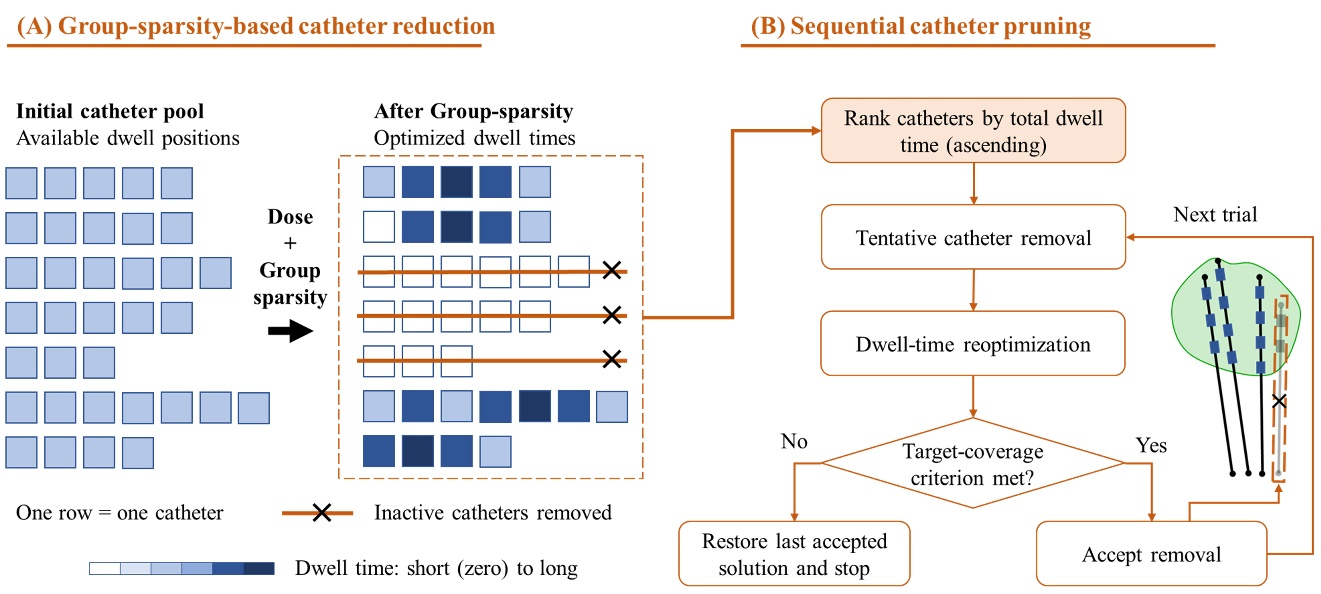
\includegraphics[width=0.92\linewidth,height=0.78\textheight,keepaspectratio]{figure4.jpg}
\caption{Adaptive catheter number determination using group-sparsity optimization and sequential pruning.}\label{fig:4}
\end{figure}

To adapt catheter-removal pressure to dosimetric performance, the global sparsity strength was initialized at $K_{0}$ = 20 and increased between blocks typically comprising 500 iterations:

\begin{equation}\label{eq:7}
K \leftarrow K(1 + \frac{0.2}{1 + 5\varepsilon_{\max}})
\end{equation}

Here, $\varepsilon_{\max}$ is the maximum relative violation among active HR-CTV and OAR dose objectives with positive weights and valid dose-volume histogram (DVH) metrics. Larger violations slowed the increase in sparsity strength.

All dwell times in the initial catheter pool were initialized to 1 s so that all catheters were initially active. FISTA used groupwise proximal updates with backtracking. Following each update of $K$, the first 50 iterations of the next block served as a stabilization period without convergence assessment. The initial block ran in full, whereas subsequent blocks could terminate early following repeated line-search failures outside stabilization.

To safeguard HR-CTV coverage during the Group-sparsity stage, feasibility was assessed by dose-only dwell-time reoptimization using the bound-constrained limited-memory Broyden--Fletcher--Goldfarb--Shanno (L-BFGS-B) algorithm,\cite{ref75,ref76} with nonnegative bounds and a limit of 50 iterations. Checks were performed after the first stabilization period and thereafter only when the active catheter count decreased. A configuration passed if the relative violation of the HR-CTV D\textsubscript{90} lower bound was at most 5\%, an empirical tolerance permitting exploration of further catheter reduction. Successful checks saved the active set and FISTA dwell times as the latest feasible anchor; L-BFGS-B dwell times were used only for assessment. An initial failure terminated FISTA, whereas a later failure restored the latest feasible anchor and ended the run. In addition to a failed feasibility check, stopping criteria included three consecutive eligible block-end comparisons without an active-set change or reaching 20,000 iterations. Comparisons were eligible only if the active set had remained unchanged for at least 10 iterations and the final iteration had no line-search failure.

Following the Group-sparsity stage, sequential pruning was performed to explore further catheter reduction, as shown in Figure~\ref{fig:4}(B). Catheters were ranked once in ascending order of total dwell time in the final FISTA solution. The cumulative dwell time of removed catheters was capped at 5\% of that solution's total dwell time, with the ranking and cap fixed throughout Pruning. The same dose-only reoptimization was applied to the complete active set before Pruning and after each tentative removal. Removal was accepted only if the dose-only objective value was finite and the relative violation of the HR-CTV D\textsubscript{90} lower bound was at most 5\%; otherwise, the last accepted solution was restored and Pruning stopped. Pruning also stopped when the cumulative removal limit was reached or only one catheter remained.

\subsubsection{Catheter Spatial Configuration Optimization}\label{sec:2-1-3}

Starting from the configuration retained after Pruning, spatial configuration optimization sought to improve the dose distribution while maintaining the determined catheter count. It comprised simulated annealing (SA)-based catheter exchange followed by local geometric fine-tuning. Both steps minimized the sum of the dose terms in Equation~\eqref{eq:5} and a dwell-time smoothness penalty that discourages abrupt changes between adjacent dwell times:

\begin{equation}\label{eq:8}
F_{\text{smooth}}\left( t \right) = \frac{\lambda_{\text{smooth}}}{2}\sum_{c = 1}^{C}{\sum_{j = 1}^{n_{c} - 1}\left( t_{c,j + 1} - t_{c,j} \right)^{2}}
\end{equation}

Here, $C$ is the retained catheter count, $t_{c,j}$ denotes the dwell time at position $j$ of catheter $c$, $n_{c}$ is its number of dwell positions, and $\lambda_{\text{smooth}}$ = 1.

Before each step, L-BFGS-B reoptimized dwell times using the dose-plus-smoothness objective to establish a baseline. Each proposed configuration was first checked for geometric feasibility. For feasible proposals, L-BFGS-B reoptimized dwell times for all catheters before objective evaluation, allowing each configuration to be assessed with an adapted dwell-time distribution. Both steps used the Metropolis acceptance criterion,\cite{ref77} allowing probabilistic acceptance of objective increases, and retained their respective lowest-objective solutions.

To explore alternative catheter combinations across the full feasible candidate set, each SA iteration replaced one randomly selected catheter with a candidate not already present in the current configuration, as illustrated in Figure~\ref{fig:5}(A). A proposal required valid dwell positions within the HR-CTV and at least 2-mm separation from the remaining catheters. The initial temperature was $T_{0} = max(10^{- 6},0.3F_{0})$, where $F_{0}$ was the baseline objective value after dwell-time reoptimization, and the temperature was reduced by a factor of 0.95 at each iteration. SA stopped after at most 1,000 iterations or 50 consecutive iterations without improvement in the best objective value.

\FloatBarrier
\begin{figure}[H]
\centering
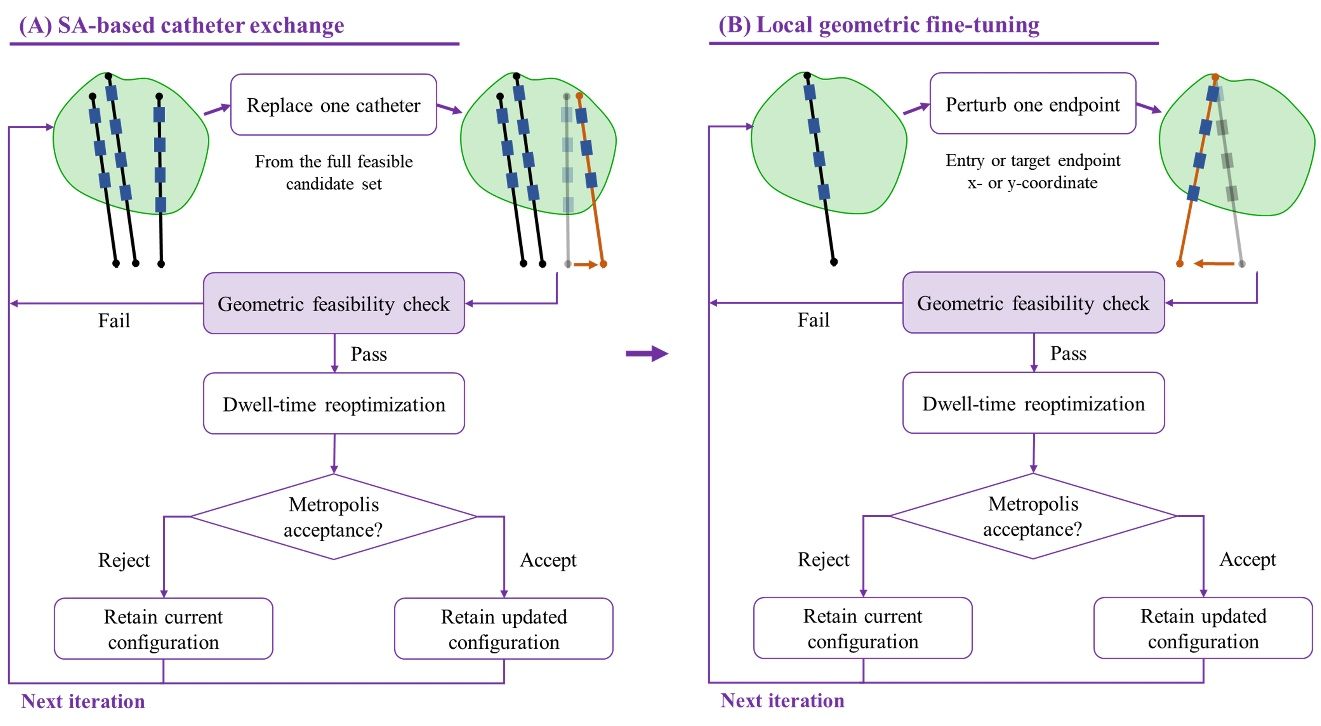
\includegraphics[width=0.92\linewidth,height=0.78\textheight,keepaspectratio]{figure5.jpg}
\caption{Catheter spatial configuration optimization using SA-based catheter exchange and local geometric fine-tuning. Gray and orange trajectories indicate the original and proposed paths, respectively. Both steps hold catheter count constant and reoptimize dwell times for feasible proposals.}\label{fig:5}
\end{figure}

Starting from the configuration retained during SA, Fine-tuning explored neighboring configurations without restricting trajectories to the sampled candidate set, as shown in Figure~\ref{fig:5}(B). At each iteration, one catheter was randomly selected, and the \emph{x}- or \emph{y}-coordinate of either its entry or target endpoint was perturbed uniformly within \ensuremath{\pm}1/50 of the corresponding sampling-plane extent along that axis. After perturbation, the target-side endpoint was reset to the HR-CTV surface by truncating or extending the updated trajectory. Proposals violating the candidate-generation geometric constraints or the 2-mm inter-catheter separation were rejected. Dwell positions were regenerated for geometrically feasible trajectories, and proposals without valid HR-CTV dwell positions were also rejected. Fine-tuning used an empirically selected initial temperature of 100 and the same cooling schedule as SA. It stopped after at most 1,000 iterations or when more than 50 consecutive feasible perturbations had been rejected.

\subsection{Evaluation Framework}\label{sec:2-2}

\subsubsection{Patient Cohort and Clinical Planning}\label{sec:2-2-1}

This retrospective study included 94 fraction plans from 26 patients with locally recurrent cervical cancer treated at Peking University Third Hospital between November 2017 and April 2023, all of whom had received prior pelvic external beam radiotherapy. The median number of included fractions per patient was 3 (interquartile range [IQR], 3--5; range, 1--7). The median HR-CTV volume was 53 cm\textsuperscript{3} (IQR, 33--73; range, 14--247). The median number of clinical catheters per fraction was 6 (IQR, 5--7; range, 3--11). Eligibility required that, after normalization of each clinical plan to an HR-CTV D\textsubscript{90} of 600 cGy, all applicable OAR dose limits were satisfied: bladder D\textsubscript{2cc} \ensuremath{\leq} 550 cGy; rectum, colon, and small-intestine D\textsubscript{2cc} \ensuremath{\leq} 430 cGy; and urethral D\textsubscript{0.1cc} \ensuremath{\leq} 550 cGy. These institutional dose limits were informed by EMBRACE II\cite{ref78}. Due to anatomical variability, not all OARs were considered clinically relevant for dosimetric evaluation and contoured in every fraction. OARs without available contours were excluded from both eligibility assessment and automated optimization.

Patients underwent individualized template-guided interstitial brachytherapy at 6 Gy per fraction, with computed tomography (CT) simulation and structure delineation performed for each fraction. Post-insertion CT scans were acquired with the template and catheters in place (Brilliance Big Bore, Philips Healthcare, Cleveland, OH, USA; 120 kV, 150 mA, 3-mm slices). The gross tumor volume (GTV) was delineated based on CT-visible disease, with reference to diagnostic imaging and clinical examination. The HR-CTV included the GTV plus a margin of 0.3--0.5 cm. In cases with uterine corpus or vaginal involvement, the HR-CTV also included 3/4 of the uterine corpus or the entire vagina, thereby expanding the target volume to encompass surrounding tissues. Clinical plans were generated using Eclipse 15.5 (Varian Medical Systems, USA) with volume-based optimization and dose shaper tools. All plans were prepared by a medical physicist with more than 10 years of experience following institutional protocols based on EMBRACE II\cite{ref78} and reviewed and approved by a senior radiation oncologist with more than 15 years of experience before treatment. The study was approved by the Ethics Committee of Peking University Third Hospital (approval No. IRB00006761-M2019210).

\subsubsection{Evaluation Design and Statistical Analysis}\label{sec:2-2-2}

The final automated plans were compared with the clinical plans to evaluate catheter reduction and dosimetric performance. Stage-wise comparisons assessed clinical versus Group-sparsity, Group-sparsity versus Pruning, Pruning versus SA, and SA versus Fine-tuning. Dosimetric comparisons across the four automated optimization stages used dwell times optimized with the same dose-plus-smoothness objective. For Group-sparsity and Pruning, independent dwell-time reoptimizations were performed with the retained catheter configurations fixed; these evaluations did not affect subsequent optimization. SA and Fine-tuning metrics were obtained from their respective retained best solutions.

Sampling points consisted of structure-overlapping voxels weighted by fractional structure volume. AAPM TG-43 unit-time dose rates\cite{ref79} were calculated dynamically for each configuration using an NVIDIA GeForce RTX 2080 Ti GPU, while optimization ran on an Intel Xeon E5-2620 v4 CPU. For each fraction, clinical and automated plans were evaluated using the same TG-43 dose-rate model and source strength. Procedure-specific random seeds were fixed across experimental configurations.

The Reference configuration used the 30\textdegree{} azimuthal constraint, dose-guided core selection with random supplementation, and sparsity-weight multipliers of 0.7 and 1.5 for core and supplementary catheters, respectively. The azimuthal threshold was specified based on clinical experience, whereas the sparsity-weight multipliers were selected based on preliminary testing. Azimuth-disabled omitted the azimuthal constraint during candidate generation and Fine-tuning checks. Uniform-weight used the Reference initial catheter pool with a multiplier of 1.0 for all catheters; Random-pool constructed the initial pool from the same eligible candidate set in random order under the same geometric criteria and pool limit, also using a multiplier of 1.0.

Ablation comparisons assessed the azimuthal constraint (Reference versus Azimuth-disabled), differential sparsity weighting (Reference versus Uniform-weight), initial-pool construction (Uniform-weight versus Random-pool), and the combined effects of pool construction and weighting (Reference versus Random-pool). All other data, objectives, and settings were held constant.

Dosimetric metrics included HR-CTV D\textsubscript{95}, V\textsubscript{150}, and V\textsubscript{200}; bladder, rectum, colon, and small-intestine D\textsubscript{2cc}; and urethral D\textsubscript{0.1cc}. Plans were individually normalized to HR-CTV D\textsubscript{90} = 600 cGy before calculating dosimetric metrics, total dwell time, and the dwell-time smoothness penalty. Additional metrics included candidate and initial-pool counts, catheter counts after Group-sparsity and Pruning, and active dwell-position counts for SA and Fine-tuning. Computational metrics included iteration counts and termination behavior for FISTA, SA, and Fine-tuning, as well as candidate-generation, stage-specific, and total computation times. Total optimization time spanned candidate generation through Fine-tuning.

Plan metrics were summarized at the fraction-plan level as medians and IQRs. Stage-wise paired changes were calculated as the later stage minus the preceding stage. To account for multiple fractions per patient, valid fraction-level values were averaged within each patient and comparison condition, and the resulting patient-level means were compared using two-sided Wilcoxon signed-rank tests. Patients without valid paired data for a metric were excluded from that comparison. The nominal significance level was 0.05. Bonferroni correction across the five OAR metrics yielded a threshold of \emph{P} < 0.01, which was also applied to all other patient-level paired metrics.

\FloatBarrier
\section{Results}\label{sec:3}

\subsection{Clinical versus Automated Plans}\label{sec:3-1}

All 94 plans completed the automated workflow. Figure~\ref{fig:6} shows the paired catheter counts and their distributions for clinical and final automated plans. Of the 94 plans, 78 (83.0\%) used fewer catheters, 11 (11.7\%) were unchanged, and five (5.3\%) used more. Median catheter count decreased from six to four, with a median paired change of \ensuremath{-}2 (\emph{P} < 0.001).

\FloatBarrier
\begin{figure}[H]
\centering
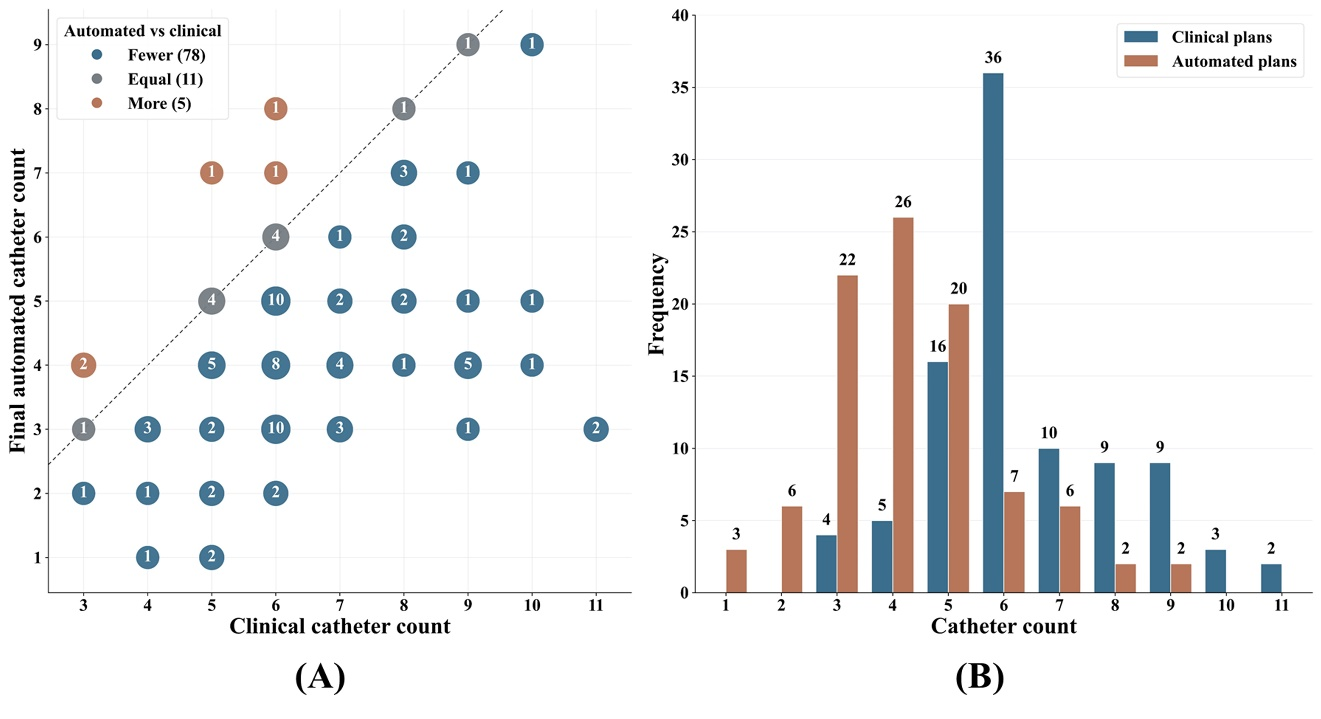
\includegraphics[width=0.92\linewidth,height=0.78\textheight,keepaspectratio]{figure6.jpg}
\caption{Clinical versus final automated catheter counts. (A) Joint-frequency bubble plot. Circle area and the number inside indicate the frequency of each catheter-count combination; the dashed line indicates equal catheter counts. (B) Marginal-frequency distributions of clinical and final automated catheter counts. Bar heights and labels indicate the number of fraction plans at each catheter count.}\label{fig:6}
\end{figure}

After normalization to HR-CTV D\textsubscript{90} = 600 cGy, HR-CTV D\textsubscript{95} decreased by a median of 5.7 cGy (\emph{P} = 0.002). Colon D\textsubscript{2cc} and urethral D\textsubscript{0.1cc} decreased by 3.3 cGy (\emph{P} = 0.008) and 15.7 cGy (\emph{P} < 0.001), respectively. Differences in HR-CTV V\textsubscript{150} and V\textsubscript{200}, the other OAR dose metrics, and total dwell time did not meet the prespecified significance threshold. Of the 94 final automated plans, 93 met all applicable institutional OAR dose limits. In the remaining fraction, bladder D\textsubscript{2cc} increased from 526.7 to 568.5 cGy (limit, 550 cGy), and rectum D\textsubscript{2cc} increased from 412.5 to 453.8 cGy (limit, 430 cGy), compared with the corresponding clinical plan. Table~\ref{tab:1} summarizes the clinical and final automated plan metrics.

\begin{table}[H]
\centering
\small\setstretch{1}
\setlength{\tabcolsep}{3pt}
\renewcommand{\arraystretch}{1.1}
\caption{Clinical and final automated plan metrics. Paired changes were calculated at the fraction-plan level as final automated minus clinical. \emph{P} values were obtained from patient-level comparisons. Values are medians (IQRs), except for P values and patient/fraction counts.}\label{tab:1}
\begin{tabularx}{\textwidth}{@{}>{\raggedright\arraybackslash}p{0.18\textwidth}*{3}{>{\raggedright\arraybackslash}X}>{\raggedright\arraybackslash}p{0.08\textwidth}>{\raggedright\arraybackslash}p{0.12\textwidth}@{}}
\toprule
\textbf{\textbf{Metric}} & \textbf{\textbf{Clinical plans}} & \textbf{\textbf{Final automated plans}} & \textbf{\textbf{Paired change}} & \textbf{\textbf{\emph{P} value}} & \textbf{\textbf{Patients\newline /fractions}} \\
\midrule
Number of catheters & 6 (5 to 7) & 4 (3 to 5) & \ensuremath{-}2 (\ensuremath{-}3 to \ensuremath{-}1) & <0.001 & 26/94 \\
HR-CTV D\textsubscript{95}, cGy & 542.4 (533.1 to 548.9) & 538.2 (527.9 to 543.8) & \ensuremath{-}5.7 (\ensuremath{-}12.3 to 2.2) & 0.002 & 26/94 \\
HR-CTV V\textsubscript{150}, \% & 55.0 (51.7 to 57.2) & 55.9 (53.2 to 58.0) & 1.3 (\ensuremath{-}1.8 to 2.9) & 0.020 & 26/94 \\
HR-CTV V\textsubscript{200}, \% & 31.2 (26.5 to 34.5) & 31.0 (25.2 to 35.0) & 0.5 (\ensuremath{-}4.0 to 4.1) & 0.568 & 26/94 \\
Bladder D\textsubscript{2cc}, cGy & 430.3 (351.3 to 464.3) & 423.9 (325.4 to 463.4) & \ensuremath{-}1.8 (\ensuremath{-}11.4 to 2.8) & 0.096 & 26/94 \\
Rectum D\textsubscript{2cc}, cGy & 367.9 (329.2 to 394.8) & 363.3 (325.6 to 393.3) & \ensuremath{-}0.4 (\ensuremath{-}6.9 to 4.2) & 0.058 & 26/94 \\
Colon D\textsubscript{2cc}, cGy & 185.3 (105.2 to 323.8) & 183.4 (101.0 to 314.9) & \ensuremath{-}3.3 (\ensuremath{-}9.0 to 0.4) & 0.008 & 19/57 \\
Small intestine D\textsubscript{2cc}, cGy & 133.2 (103.5 to 170.9) & 121.0 (102.3 to 183.4) & \ensuremath{-}5.2 (\ensuremath{-}14.4 to \ensuremath{-}0.7) & 0.248 & 11/19 \\
Urethra D\textsubscript{0.1cc}, cGy & 344.9 (194.7 to 446.2) & 314.0 (186.3 to 420.3) & \ensuremath{-}15.7 (\ensuremath{-}31.1 to \ensuremath{-}5.8) & <0.001 & 25/90 \\
Total dwell time, s & 246.4 (184.3 to 295.2) & 244.0 (177.2 to 301.3) & 2.2 (\ensuremath{-}7.3 to 14.1) & 0.107 & 26/94 \\
\bottomrule
\end{tabularx}
\end{table}

\subsection{Stage-Wise Results and Computation Time}\label{sec:3-2}

Candidate generation reached 3,000 feasible trajectories in all 94 plans. The median initial catheter pool contained 62 catheters (IQR, 56 to 68). Median counts were 2.5 core catheters (IQR, 1 to 3) and 60 supplementary catheters (IQR, 55 to 64).

The median catheter count after Group-sparsity was five, compared with six in the clinical plans; the paired difference did not meet the prespecified significance threshold (\emph{P} = 0.016). Relative to the clinical plans, HR-CTV D\textsubscript{95} decreased by a median of 3.8 cGy (\emph{P} = 0.007), and urethral D\textsubscript{0.1cc} decreased by 10.3 cGy (\emph{P} < 0.001). Pruning reduced median catheter count further to four (\emph{P} < 0.001 versus Group-sparsity). Relative to the Group-sparsity stage, HR-CTV D\textsubscript{95} decreased by 1.7 cGy; V\textsubscript{150} and V\textsubscript{200} increased by 1.0 and 1.6 percentage points; all evaluated OAR dose metrics increased; and total dwell time increased by 4.7 s (all \emph{P} < 0.01).

\begin{table}[H]
\centering
\small\setstretch{1}
\setlength{\tabcolsep}{3pt}
\renewcommand{\arraystretch}{1.1}
\caption{Catheter counts, dosimetric indices, and dwell-time characteristics of clinical plans and automated plans after Group-sparsity, Pruning, SA, and Fine-tuning. Values are medians (IQRs).}\label{tab:2}
\begin{tabularx}{\textwidth}{@{}>{\raggedright\arraybackslash}p{0.18\textwidth}*{5}{>{\raggedright\arraybackslash}X}@{}}
\toprule
\textbf{\textbf{Metric}} & \textbf{\textbf{Clinical}} & \textbf{\textbf{Group-sparsity}} & \textbf{\textbf{Pruning}} & \textbf{\textbf{SA}} & \textbf{\textbf{Fine-tuning}} \\
\midrule
Number of catheters & 6 (5 to 7) & 5 (4 to 6) & 4 (3 to 5) & 4 (3 to 5) & 4 (3 to 5) \\
HR-CTV D\textsubscript{95}, cGy & 542.4 (533.1 to 548.9) & 537.2 (528.9 to 543.6) & 533.9 (526.0 to 540.5) & 537.3 (529.9 to 544.2) & 538.2 (527.9 to 543.8) \\
HR-CTV V\textsubscript{150}, \% & 55.0 (51.7 to 57.2) & 55.1 (51.8 to 57.3) & 56.2 (53.9 to 58.9) & 55.5 (52.7 to 57.8) & 55.9 (53.2 to 58.0) \\
HR-CTV V\textsubscript{200}, \% & 31.2 (26.5 to 34.5) & 31.7 (25.2 to 34.9) & 33.0 (28.6 to 36.9) & 31.5 (25.0 to 34.8) & 31.0 (25.2 to 35.0) \\
Bladder D\textsubscript{2cc}, cGy & 430.3 (351.3 to 464.3) & 424.0 (324.7 to 470.2) & 429.5 (334.4 to 472.9) & 423.9 (330.8 to 464.7) & 423.9 (325.4 to 463.4) \\
Rectum D\textsubscript{2cc}, cGy & 367.9 (329.2 to 394.8) & 364.0 (324.1 to 394.8) & 373.0 (328.9 to 405.3) & 368.2 (325.6 to 393.4) & 363.3 (325.6 to 393.3) \\
Colon D\textsubscript{2cc}, cGy & 185.3 (105.2 to 323.8) & 186.4 (103.5 to 313.6) & 192.6 (104.9 to 317.9) & 183.5 (100.2 to 316.0) & 183.4 (101.0 to 314.9) \\
Small intestine D\textsubscript{2cc}, cGy & 133.2 (103.5 to 170.9) & 120.4 (101.4 to 177.1) & 124.7 (101.5 to 186.2) & 119.5 (102.8 to 181.7) & 121.0 (102.3 to 183.4) \\
Urethra D\textsubscript{0.1cc}, cGy & 344.9 (194.7 to 446.2) & 313.8 (183.8 to 427.4) & 319.0 (184.4 to 429.6) & 314.3 (187.2 to 421.9) & 314.0 (186.3 to 420.3) \\
Total dwell time, s & 246.4 (184.3 to 295.2) & 243.3 (178.7 to 303.1) & 247.3 (184.3 to 310.8) & 245.1 (179.9 to 311.8) & 244.0 (177.2 to 301.3) \\
Number of active dwell positions & --- & --- & --- & 38.0 (26.3 to 49.0) & 37.0 (27.0 to 49.8) \\
Dwell-time smoothness penalty & --- & --- & --- & 8.9 (3.0 to 36.2) & 5.8 (0.9 to 14.4) \\
\bottomrule
\end{tabularx}
\end{table}

At the retained catheter count, SA increased HR-CTV D\textsubscript{95} by 2.1 cGy and reduced V\textsubscript{150} and V\textsubscript{200} by 1.0 and 1.7 percentage points relative to Pruning (all \emph{P} < 0.01). Bladder, rectum, colon, and urethral dose metrics also decreased, whereas small-intestine D\textsubscript{2cc} did not differ significantly. Total dwell time decreased by 1.0 s (\emph{P} = 0.008). Fine-tuning produced no significant additional change in HR-CTV metrics or total dwell time. Rectum D\textsubscript{2cc} decreased by 1.3 cGy (\emph{P} = 0.001), and the dwell-time smoothness penalty decreased by 2.2 (\emph{P} < 0.001); active dwell-position count did not differ significantly. Tables 2 and 3 present the plan metrics across optimization stages and the paired changes between consecutive stages, respectively.

\begin{table}[H]
\centering
\footnotesize\setstretch{1}
\setlength{\tabcolsep}{3pt}
\renewcommand{\arraystretch}{1.05}
\caption{Changes between consecutive optimization stages. Each comparison cell presents the median paired change (IQR) above the \emph{P} value. Changes were calculated at the fraction-plan level as the later stage minus the preceding stage, whereas \emph{P} values were obtained from patient-level comparisons.}\label{tab:3}
\begin{tabularx}{\textwidth}{@{}>{\raggedright\arraybackslash}p{0.18\textwidth}*{4}{>{\raggedright\arraybackslash}X}>{\raggedright\arraybackslash}p{0.12\textwidth}@{}}
\toprule
\textbf{\textbf{Metric}} & \textbf{\textbf{Group-sparsity \ensuremath{-} Clinical}} & \textbf{\textbf{Pruning \ensuremath{-} Group-sparsity}} & \textbf{\textbf{SA \ensuremath{-} Pruning}} & \textbf{\textbf{Fine-tuning \ensuremath{-} SA}} & \textbf{\textbf{Patients\newline /fractions}} \\
\midrule
Number of catheters & \ensuremath{-}1 (\ensuremath{-}3 to 1)\newline \emph{P} = 0.016 & \ensuremath{-}1 (\ensuremath{-}1 to 0)\newline \emph{P} < 0.001 & 0 (0 to 0)\newline --- & 0 (0 to 0)\newline --- & 26/94 \\
HR-CTV D\textsubscript{95}, cGy & \ensuremath{-}3.8 (\ensuremath{-}12.4 to 3.6)\newline \emph{P} = 0.007 & \ensuremath{-}1.7 (\ensuremath{-}7.8 to 0.8)\newline \emph{P} = 0.001 & 2.1 (\ensuremath{-}1.0 to 6.6)\newline \emph{P} = 0.001 & 0.5 (\ensuremath{-}2.1 to 2.5)\newline \emph{P} = 0.770 & 26/94 \\
HR-CTV V\textsubscript{150}, \% & 0.0 (\ensuremath{-}1.8 to 2.5)\newline \emph{P} = 0.144 & 1.0 (0.0 to 2.4)\newline \emph{P} < 0.001 & \ensuremath{-}1.0 (\ensuremath{-}2.6 to 0.0)\newline \emph{P} = 0.003 & 0.1 (\ensuremath{-}0.4 to 0.8)\newline \emph{P} = 0.424 & 26/94 \\
HR-CTV V\textsubscript{200}, \% & 0.3 (\ensuremath{-}2.8 to 4.1)\newline \emph{P} = 0.424 & 1.6 (0.0 to 3.3)\newline \emph{P} < 0.001 & \ensuremath{-}1.7 (\ensuremath{-}4.2 to 0.0)\newline \emph{P} < 0.001 & 0.0 (\ensuremath{-}0.9 to 0.8)\newline \emph{P} = 0.424 & 26/94 \\
Bladder D\textsubscript{2cc}, cGy & \ensuremath{-}0.7 (\ensuremath{-}12.4 to 9.3)\newline \emph{P} = 0.770 & 4.3 (\ensuremath{-}0.8 to 10.2)\newline \emph{P} = 0.002 & \ensuremath{-}5.8 (\ensuremath{-}15.6 to 0.0)\newline \emph{P} = 0.001 & \ensuremath{-}0.3 (\ensuremath{-}3.6 to 1.5)\newline \emph{P} = 0.016 & 26/94 \\
Rectum D\textsubscript{2cc}, cGy & 1.1 (\ensuremath{-}7.1 to 10.6)\newline \emph{P} = 0.869 & 2.5 (\ensuremath{-}1.3 to 9.9)\newline \emph{P} = 0.001 & \ensuremath{-}3.1 (\ensuremath{-}10.9 to 0.0)\newline \emph{P} = 0.002 & \ensuremath{-}1.3 (\ensuremath{-}4.3 to 0.4)\newline \emph{P} = 0.001 & 26/94 \\
Colon D\textsubscript{2cc}, cGy & \ensuremath{-}2.9 (\ensuremath{-}11.4 to 3.8)\newline \emph{P} = 0.064 & 1.9 (\ensuremath{-}0.1 to 5.8)\newline \emph{P} = 0.003 & \ensuremath{-}3.2 (\ensuremath{-}8.4 to \ensuremath{-}0.5)\newline \emph{P} < 0.001 & \ensuremath{-}0.1 (\ensuremath{-}1.7 to 0.4)\newline \emph{P} = 0.053 & 19/57 \\
Small intestine D\textsubscript{2cc}, cGy & \ensuremath{-}8.0 (\ensuremath{-}15.8 to 1.2)\newline \emph{P} = 0.213 & 2.3 (0.0 to 3.9)\newline \emph{P} = 0.003 & \ensuremath{-}2.8 (\ensuremath{-}6.6 to 0.0)\newline \emph{P} = 0.022 & \ensuremath{-}0.4 (\ensuremath{-}2.2 to 0.1)\newline \emph{P} = 0.575 & 11/19 \\
Urethra D\textsubscript{0.1cc}, cGy & \ensuremath{-}10.3 (\ensuremath{-}26.1 to \ensuremath{-}3.5)\newline \emph{P} < 0.001 & 1.4 (\ensuremath{-}0.9 to 6.1)\newline \emph{P} = 0.002 & \ensuremath{-}4.3 (\ensuremath{-}10.4 to 0.0)\newline \emph{P} = 0.003 & \ensuremath{-}0.9 (\ensuremath{-}4.4 to 1.4)\newline \emph{P} = 0.074 & 25/90 \\
Total dwell time, s & 0.7 (\ensuremath{-}8.1 to 14.2)\newline \emph{P} = 0.191 & 4.7 (0.2 to 9.5)\newline \emph{P} < 0.001 & \ensuremath{-}1.0 (\ensuremath{-}9.3 to 2.6)\newline \emph{P} = 0.008 & \ensuremath{-}0.2 (\ensuremath{-}2.7 to 1.7)\newline \emph{P} = 0.049 & 26/94 \\
Number of active dwell positions & --- & --- & --- & 0.0 (0.0 to 1.0)\newline \emph{P} = 0.047 & 26/94 \\
Dwell-time smoothness penalty & --- & --- & --- & \ensuremath{-}2.2 (\ensuremath{-}9.0 to \ensuremath{-}0.4)\newline \emph{P} < 0.001 & 26/94 \\
\bottomrule
\end{tabularx}
\end{table}

Median total optimization time was 510.6 s. Median times for Group-sparsity, SA, and Fine-tuning were 230.1, 86.7, and 163.8 s, respectively. FISTA stopped at the active-set stability criterion in 92 plans and at the HR-CTV coverage safeguard in two; none reached 20,000 iterations. All SA runs stopped before 1,000 iterations. Fine-tuning reached 1,000 iterations in one plan. Table~\ref{tab:4} summarizes the iteration counts and computation times across optimization stages.

\begin{table}[H]
\centering
\small\setstretch{1}
\setlength{\tabcolsep}{3pt}
\renewcommand{\arraystretch}{1.1}
\caption{Optimization iterations and computation time. Values are medians (IQRs).}\label{tab:4}
\begin{tabularx}{\textwidth}{@{}>{\raggedright\arraybackslash}p{0.30\textwidth}*{2}{>{\raggedright\arraybackslash}X}@{}}
\toprule
\textbf{\textbf{Metric}} & \textbf{\textbf{Iterations}} & \textbf{\textbf{Runtime, s}} \\
\midrule
Candidate generation & --- & 3.4 (2.5 to 4.5) \\
Initial pool construction & --- & 3.0 (2.4 to 4.3) \\
Group-sparsity & 4434.5 (3523.3 to 6291.3) & 230.1 (151.0 to 371.1) \\
Pruning & --- & 0.9 (0.4 to 1.4) \\
SA & 176 (129.5 to 240.0) & 86.7 (64.0 to 122.6) \\
Fine-tuning & 312.5 (253.0 to 444.0) & 163.8 (115.2 to 230.1) \\
Total optimization & --- & 510.6 (405.9 to 734.5) \\
\bottomrule
\end{tabularx}
\end{table}

\FloatBarrier
\subsection{Ablation Studies}\label{sec:3-3}

All 94 plans completed the workflow under each evaluated configuration. The analyses examined the effects of the azimuthal constraint, initial-pool construction, and sparsity-weight configuration on the final catheter configurations and plan quality.

\subsubsection{Azimuthal Constraint}\label{sec:3-3-1}

Disabling the azimuthal constraint reduced the median initial catheter pool from 62 to 37.5 catheters (median paired change, \ensuremath{-}25; \emph{P} < 0.001), without a significant change in catheter count after Group-sparsity or in the final plan. Final HR-CTV V\textsubscript{200} increased by 1.2 percentage points (\emph{P} = 0.003), and total optimization time decreased by 89.5 s (\emph{P} = 0.007). Other final dose metrics and total dwell time did not differ significantly. Table~\ref{tab:5} summarizes the ablation results for the azimuthal constraint. Four fraction plans from different patients were selected for visual comparison; each had at least six final catheters in both configurations, with the counts differing by no more than two. Figure~\ref{fig:7} shows the corresponding catheter configurations with and without the azimuthal constraint.

\FloatBarrier
\begin{figure}[H]
\centering
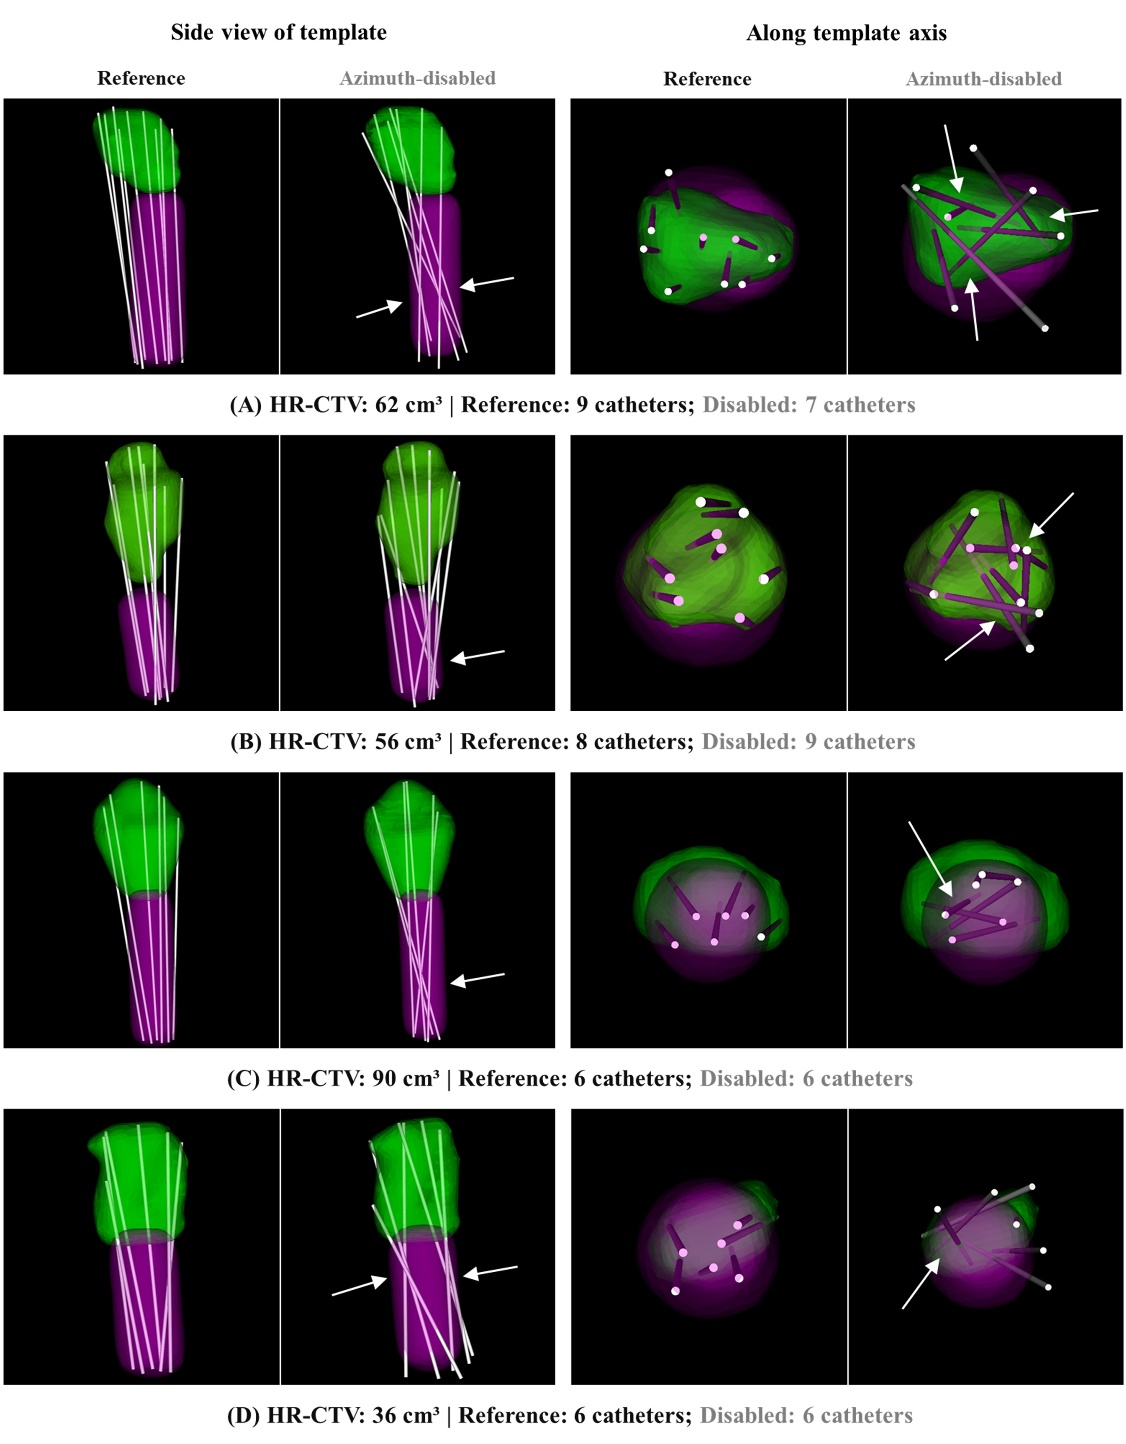
\includegraphics[width=0.85\linewidth,height=0.68\textheight,keepaspectratio]{figure7.jpg}
\caption{Final catheter configurations with and without the azimuthal constraint. Four selected fraction plans are shown in side and axial views of the template. HR-CTV volumes and final catheter counts are indicated for each plan. White arrows indicate projected crossings between catheter trajectories in the Azimuth-disabled configurations.}\label{fig:7}
\end{figure}

\begin{table}[!htbp]
\centering
\small\setstretch{1}
\setlength{\tabcolsep}{3pt}
\renewcommand{\arraystretch}{1.1}
\caption{Ablation results for the azimuthal constraint. Paired changes were calculated at the fraction-plan level as Azimuth-disabled minus Reference. \emph{P} values were obtained from patient-level comparisons. Values are medians (IQRs), except for P values and patient/fraction counts.}\label{tab:5}
\begin{tabularx}{\textwidth}{@{}>{\raggedright\arraybackslash}p{0.18\textwidth}*{3}{>{\raggedright\arraybackslash}X}>{\raggedright\arraybackslash}p{0.08\textwidth}>{\raggedright\arraybackslash}p{0.12\textwidth}@{}}
\toprule
\textbf{\textbf{Metric}} & \textbf{\textbf{Reference}} & \textbf{\textbf{Azimuth-disabled}} & \textbf{\textbf{Paired change}} & \textbf{\textbf{\emph{P} value}} & \textbf{\textbf{Patients\newline /fractions}} \\
\midrule
Initial catheter pool size & 62 (56 to 68) & 37.5 (34 to 40) & \ensuremath{-}25 (\ensuremath{-}28 to \ensuremath{-}21) & <0.001 & 26/94 \\
Number of active catheters after Group-sparsity & 5 (4 to 6) & 5 (3 to 7) & 0 (\ensuremath{-}1 to 1) & 0.538 & 26/94 \\
Final catheter number & 4 (3 to 5) & 4 (3 to 5) & 0 (\ensuremath{-}1 to 1) & 0.437 & 26/94 \\
HR-CTV D\textsubscript{95}, cGy & 538.2 (527.9 to 543.8) & 537.9 (530.0 to 545.8) & 0.9 (\ensuremath{-}4.3 to 6.7) & 0.603 & 26/94 \\
HR-CTV V\textsubscript{150}, \% & 55.9 (53.2 to 58.0) & 56.8 (54.1 to 58.4) & 0.6 (\ensuremath{-}0.5 to 2.2) & 0.023 & 26/94 \\
HR-CTV V\textsubscript{200}, \% & 31.0 (25.2 to 35.0) & 33.2 (28.3 to 36.7) & 1.2 (\ensuremath{-}0.5 to 4.5) & 0.003 & 26/94 \\
Bladder D\textsubscript{2cc}, cGy & 423.9 (325.4 to 463.4) & 422.7 (323.8 to 463.0) & \ensuremath{-}0.6 (\ensuremath{-}5.8 to 4.6) & 0.469 & 26/94 \\
Rectum D\textsubscript{2cc}, cGy & 363.3 (325.6 to 393.3) & 359.8 (324.0 to 397.9) & \ensuremath{-}0.8 (\ensuremath{-}4.7 to 4.9) & 0.409 & 26/94 \\
Colon D\textsubscript{2cc}, cGy & 183.4 (101.0 to 314.9) & 182.5 (102.1 to 309.0) & 0.2 (\ensuremath{-}3.0 to 2.6) & 0.748 & 19/57 \\
Small intestine D\textsubscript{2cc}, cGy & 121.0 (102.3 to 183.4) & 118.0 (101.4 to 186.7) & 1.2 (\ensuremath{-}1.3 to 3.4) & 0.155 & 11/19 \\
Urethra D\textsubscript{0.1cc}, cGy & 314.0 (186.3 to 420.3) & 314.3 (193.2 to 421.3) & 1.1 (\ensuremath{-}4.0 to 8.2) & 0.397 & 25/90 \\
Total dwell time, s & 244.0 (177.2 to 301.3) & 239.9 (181.6 to 313.0) & 4.0 (\ensuremath{-}6.4 to 10.5) & 0.144 & 26/94 \\
Total optimization time, s & 510.6 (405.9 to 734.5) & 443.7 (372.8 to 584.6) & \ensuremath{-}89.5 (\ensuremath{-}190.4 to 37.1) & 0.007 & 26/94 \\
\bottomrule
\end{tabularx}
\end{table}

\subsubsection{Initial Pool and Sparsity Weights}\label{sec:3-3-2}

Reference and Uniform-weight used identical initial catheter pools. Relative to Reference, Uniform-weight increased the median final catheter count from four to five (median paired change, +1; \emph{P} = 0.002). HR-CTV V\textsubscript{200}, colon D\textsubscript{2cc}, and total dwell time decreased by 1.6 percentage points, 1.8 cGy, and 5.3 s, respectively (all \emph{P} < 0.01). The increase in active catheter count immediately after Group-sparsity did not meet the significance threshold (\emph{P} = 0.013).

Uniform-weight and Random-pool did not differ significantly in catheter count, dosimetry, total dwell time, or optimization time. Relative to Reference, Random-pool increased the median final catheter count from four to five (\emph{P} = 0.009) and decreased total dwell time by 3.9 s (\emph{P} = 0.005), without significant changes in final dose metrics or optimization time. Tables 6 and 7 present the plan metrics for the three configurations and their paired comparisons, respectively.

\begin{table}[!htbp]
\centering
\small\setstretch{1}
\setlength{\tabcolsep}{3pt}
\renewcommand{\arraystretch}{1.1}
\caption{Plan metrics by initial-pool construction and sparsity-weight configuration. Values are medians (IQRs).}\label{tab:6}
\begin{tabularx}{\textwidth}{@{}>{\raggedright\arraybackslash}p{0.30\textwidth}*{3}{>{\raggedright\arraybackslash}X}@{}}
\toprule
\textbf{\textbf{Metric}} & \textbf{\textbf{Reference}} & \textbf{\textbf{Uniform-weight}} & \textbf{\textbf{Random-pool}} \\
\midrule
Initial catheter pool size & 62 (56 to 68) & 62 (56 to 68) & 63 (58 to 66) \\
Number of active catheters after Group-sparsity & 5 (4 to 6) & 6 (5 to 7) & 5 (4 to 7) \\
Final catheter number & 4 (3 to 5) & 5 (4 to 6) & 5 (4 to 6) \\
HR-CTV D\textsubscript{95}, cGy & 538.2 (527.9 to 543.8) & 537.0 (525.7 to 545.5) & 539.5 (527.7 to 545.8) \\
HR-CTV V\textsubscript{150}, \% & 55.9 (53.2 to 58.0) & 55.4 (52.6 to 57.4) & 55.4 (52.1 to 57.7) \\
HR-CTV V\textsubscript{200}, \% & 31.0 (25.2 to 35.0) & 28.7 (23.9 to 32.6) & 28.6 (24.9 to 33.8) \\
Bladder D\textsubscript{2cc}, cGy & 423.9 (325.4 to 463.4) & 418.6 (320.4 to 459.9) & 417.3 (317.9 to 462.5) \\
Rectum D\textsubscript{2cc}, cGy & 363.3 (325.6 to 393.3) & 358.2 (319.2 to 393.4) & 359.2 (321.8 to 392.5) \\
Colon D\textsubscript{2cc}, cGy & 183.4 (101.0 to 314.9) & 183.6 (99.1 to 305.5) & 183.1 (98.7 to 309.2) \\
Small intestine D\textsubscript{2cc}, cGy & 121.0 (102.3 to 183.4) & 117.3 (101.5 to 187.5) & 120.4 (100.8 to 179.3) \\
Urethra D\textsubscript{0.1cc}, cGy & 314.0 (186.3 to 420.3) & 314.2 (186.1 to 419.2) & 308.3 (186.2 to 417.3) \\
Total dwell time, s & 244.0 (177.2 to 301.3) & 237.4 (172.6 to 301.5) & 230.9 (174.1 to 301.0) \\
Total optimization time, s & 510.6 (405.9 to 734.5) & 555.9 (436.3 to 714.3) & 508.6 (412.6 to 703.9) \\
\bottomrule
\end{tabularx}
\end{table}

\begin{table}[!htbp]
\centering
\small\setstretch{1}
\setlength{\tabcolsep}{3pt}
\renewcommand{\arraystretch}{1.1}
\caption{Paired comparisons of initial-pool construction and sparsity-weight configurations. Each comparison cell presents the median paired change (IQR) above the \emph{P} value. Changes were calculated at the fraction-plan level in the subtraction order shown in the column headings, whereas \emph{P} values were obtained from patient-level comparisons.}\label{tab:7}
\begin{tabularx}{\textwidth}{@{}>{\raggedright\arraybackslash}p{0.18\textwidth}*{3}{>{\raggedright\arraybackslash}X}>{\raggedright\arraybackslash}p{0.12\textwidth}@{}}
\toprule
\textbf{\textbf{Metric}} & \textbf{\textbf{Uniform-weight \ensuremath{-} Reference}} & \textbf{\textbf{Random-pool \ensuremath{-} Uniform-weight}} & \textbf{\textbf{Random-pool \ensuremath{-} Reference}} & \textbf{\textbf{Patients\newline /fractions}} \\
\midrule
Initial catheter pool size & 0 (0 to 0)\newline --- & 0 (\ensuremath{-}2 to 3)\newline \emph{P} = 0.516 & 0 (\ensuremath{-}2 to 3)\newline \emph{P} = 0.516 & 26/94 \\
Number of active catheters after Group-sparsity & 1 (0 to 2)\newline \emph{P} = 0.013 & 0 (\ensuremath{-}2 to 1)\newline \emph{P} = 0.201 & 0 (\ensuremath{-}1 to 2)\newline \emph{P} = 0.082 & 26/94 \\
Final catheter number & 1 (0 to 2)\newline \emph{P} = 0.002 & 0 (\ensuremath{-}2 to 1)\newline \emph{P} = 0.269 & 1 (0 to 2)\newline \emph{P} = 0.009 & 26/94 \\
HR-CTV D\textsubscript{95}, cGy & \ensuremath{-}1.5 (\ensuremath{-}7.4 to 5.6)\newline \emph{P} = 0.809 & 1.0 (\ensuremath{-}4.6 to 8.3)\newline \emph{P} = 0.107 & 0.4 (\ensuremath{-}5.0 to 6.1)\newline \emph{P} = 0.849 & 26/94 \\
HR-CTV V\textsubscript{150}, \% & 0.0 (\ensuremath{-}2.3 to 1.8)\newline \emph{P} = 0.469 & 0.4 (\ensuremath{-}1.7 to 2.2)\newline \emph{P} = 0.137 & \ensuremath{-}0.3 (\ensuremath{-}1.9 to 2.0)\newline \emph{P} = 0.732 & 26/94 \\
HR-CTV V\textsubscript{200}, \% & \ensuremath{-}1.6 (\ensuremath{-}4.6 to 1.3)\newline \emph{P} = 0.004 & 0.7 (\ensuremath{-}3.3 to 4.3)\newline \emph{P} = 0.182 & \ensuremath{-}1.1 (\ensuremath{-}5.9 to 1.9)\newline \emph{P} = 0.030 & 26/94 \\
Bladder D\textsubscript{2cc}, cGy & \ensuremath{-}1.8 (\ensuremath{-}7.4 to 2.0)\newline \emph{P} = 0.019 & \ensuremath{-}0.1 (\ensuremath{-}5.7 to 5.1)\newline \emph{P} = 0.439 & \ensuremath{-}1.1 (\ensuremath{-}7.6 to 3.7)\newline \emph{P} = 0.269 & 26/94 \\
Rectum D\textsubscript{2cc}, cGy & \ensuremath{-}1.7 (\ensuremath{-}5.4 to 2.1)\newline \emph{P} = 0.131 & \ensuremath{-}1.1 (\ensuremath{-}5.7 to 5.0)\newline \emph{P} = 0.439 & \ensuremath{-}1.4 (\ensuremath{-}7.0 to 3.9)\newline \emph{P} = 0.209 & 26/94 \\
Colon D\textsubscript{2cc}, cGy & \ensuremath{-}1.8 (\ensuremath{-}4.8 to 0.1)\newline \emph{P} = 0.008 & 0.0 (\ensuremath{-}2.0 to 3.5)\newline \emph{P} = 0.027 & \ensuremath{-}1.4 (\ensuremath{-}4.6 to 0.9)\newline \emph{P} = 0.064 & 19/57 \\
Small intestine D\textsubscript{2cc}, cGy & \ensuremath{-}0.3 (\ensuremath{-}3.5 to 2.0)\newline \emph{P} = 0.959 & \ensuremath{-}0.7 (\ensuremath{-}2.0 to 1.9)\newline \emph{P} = 0.859 & \ensuremath{-}0.8 (\ensuremath{-}2.9 to 2.3)\newline \emph{P} = 0.534 & 11/19 \\
Urethra D\textsubscript{0.1cc}, cGy & \ensuremath{-}2.1 (\ensuremath{-}6.5 to 3.3)\newline \emph{P} = 0.668 & \ensuremath{-}0.5 (\ensuremath{-}6.9 to 4.7)\newline \emph{P} = 0.339 & \ensuremath{-}3.3 (\ensuremath{-}7.6 to 4.3)\newline \emph{P} = 0.150 & 25/90 \\
Total dwell time, s & \ensuremath{-}5.3 (\ensuremath{-}16.0 to 2.0)\newline \emph{P} < 0.001 & \ensuremath{-}0.4 (\ensuremath{-}7.8 to 7.6)\newline \emph{P} = 0.551 & \ensuremath{-}3.9 (\ensuremath{-}16.7 to 3.9)\newline \emph{P} = 0.005 & 26/94 \\
Total optimization time, s & 26.3 (\ensuremath{-}123.6 to 136.2)\newline \emph{P} = 0.675 & \ensuremath{-}20.3 (\ensuremath{-}176.5 to 113.6)\newline \emph{P} = 0.849 & \ensuremath{-}0.6 (\ensuremath{-}107.0 to 86.9)\newline \emph{P} = 0.770 & 26/94 \\
\bottomrule
\end{tabularx}
\end{table}

\section{Discussion}\label{sec:4}

The proposed workflow reduced the median catheter number from 6 in the clinical plans to 4 in the final automated plans; 78 of 94 fraction plans used fewer catheters. After normalization to the same HR-CTV D\textsubscript{90}, the automated plans showed a small but significant decrease in D\textsubscript{95}, no significant differences in V\textsubscript{150} or V\textsubscript{200}, and lower colon D\textsubscript{2cc} and urethral D\textsubscript{0.1cc}. These findings suggest that reduced catheter use was accompanied by a small trade-off in HR-CTV $D_{95}$ and dose reductions in selected OARs.

Cases with increased catheter counts or particularly large reductions warrant further discussion. Five automated plans used one or two additional catheters, possibly reflecting restrictions on accessible trajectories imposed by the predefined sampling regions and geometric constraints. Conversely, the four largest reductions occurred in large targets (HR-CTV volumes, 105.5--246.8 cm\textsuperscript{3}), with catheter counts reduced from 9--11 in the clinical plans to 3--4 in the automated plans. In these four plans, HR-CTV D\textsubscript{95} decreased by 4.4--9.4 cGy after normalization, while 12 of 17 available OAR dose comparisons showed reductions. Among these four plans, the two largest OAR dose increases occurred in the same fraction, with colon D\textsubscript{2cc} rising from 382.8 to 399.6 cGy and small-intestine D\textsubscript{2cc} from 268.6 to 305.8 cGy. Although these findings support the dosimetric feasibility of substantial catheter reduction for these large targets within the planning model, they do not establish comparable implantation robustness. Additional clinical catheters may provide greater dose-shaping flexibility and greater tolerance to insertion deviations than the 3--4-catheter configurations.\cite{ref68}

The stage-wise analysis distinguished catheter reduction from subsequent configuration optimization. The Group-sparsity stage produced a sparse configuration, although its catheter-number difference from the clinical plans did not meet the prespecified significance threshold. Pruning reduced the median catheter number from five to four but lowered HR-CTV D\textsubscript{95} and increased V\textsubscript{150}, V\textsubscript{200}, the evaluated OAR dose metrics, and total dwell time, consistent with reduced dose-shaping flexibility. With the catheter count fixed, SA increased D\textsubscript{95} and reduced V\textsubscript{150}, V\textsubscript{200}, and several OAR dose metrics, supporting configuration optimization after catheter reduction. The subsequent Fine-tuning stage had a limited effect on conventional dose--volume indices. HR-CTV metrics did not differ significantly after Fine-tuning, and rectum D\textsubscript{2cc} was the only OAR metric with a significant additional reduction. The number of active dwell positions did not differ at the prespecified significance level, whereas the dwell-time smoothness penalty decreased, indicating smoother optimized dwell-time distributions, although the clinical relevance of this change was not evaluated. The median runtimes were 163.8 s for Fine-tuning and 510.6 s for the complete workflow; the incremental benefit of Fine-tuning should be weighed against its computational cost.

The initial-pool and sparsity-weighting ablation showed that, with the dose-guided initial pool held constant, replacing differential weighting with uniform weighting increased the median final catheter count from four to five and was accompanied by lower HR-CTV V\textsubscript{200}, colon D\textsubscript{2cc}, and total dwell time. In contrast, under uniform weighting, dose-guided and random initial-pool construction did not differ significantly in catheter number, dosimetry, total dwell time, or optimization time. These findings suggest that differential sparsity weighting in Reference promoted catheter reduction within the dose-guided configuration, while the accompanying increases in selected dose metrics and total dwell time highlight a trade-off between catheter use and dosimetric performance.

The azimuthal constraint altered candidate-catheter geometry, but the final catheter number did not differ significantly between configurations. Disabling the constraint reduced the initial catheter pool size and total optimization time and increased HR-CTV V\textsubscript{200}. The smaller initial pool observed without the constraint may reflect the greater angular variability of candidate trajectories, which could cause more candidates to violate the minimum inter-catheter distance of 2 mm during initial-pool construction. In the four selected plans shown in Figure~\ref{fig:7}, enabling the azimuthal constraint produced more consistently aligned catheter trajectories with fewer apparent crossings in the projected views.

This study has several limitations. It was a single-center retrospective computational replanning study using post-implantation CT images. The generalizability of the findings to broader clinical populations remains uncertain. The automated trajectories were not used to fabricate templates or guide catheter insertion, and their prospective implementation remains to be evaluated. Not all OARs were contoured in every fraction, particularly the small intestine, which was delineated in only 19 fractions from 11 patients; the corresponding results should therefore be interpreted cautiously. Because the optimization bounds were derived from the corresponding clinical plans, planning with independently specified dose objectives was not evaluated. Several algorithmic parameters, including the 30\textdegree{} azimuthal threshold, the 5\% HR-CTV D\textsubscript{90} feasibility tolerance, the 5\% cumulative dwell-time limit for Pruning, and the perturbation magnitude used in Fine-tuning, were selected based on clinical experience. Further sensitivity analyses are needed to assess the impact of these parameter choices on planning performance. The nonconvex sparsity formulation and heuristic stopping criteria do not guarantee a globally optimal catheter configuration. Finally, the study evaluated planned dose distributions and computation time but not procedural burden, toxicity, or clinical outcomes.

\FloatBarrier
\section{Conclusions}\label{sec:5}

This study presents an integrated automated planning approach that combines catheter generation and initial-pool construction with adaptive catheter number determination and subsequent fixed-count spatial configuration and dwell-time optimization for individualized template-guided HDR-ISBT. In retrospective computational replanning, the framework reduced the median catheter number from six to four. After normalization to the same HR-CTV D\textsubscript{90}, the automated plans showed a small but statistically significant reduction in HR-CTV D\textsubscript{95}, no significant differences in V\textsubscript{150} or V\textsubscript{200}, and lower colon D\textsubscript{2cc} and urethral D\textsubscript{0.1cc} than the clinical plans. Stage-wise analysis showed that Pruning enabled further catheter reduction but adversely affected several dosimetric metrics; subsequent SA-based spatial configuration optimization mitigated several of these changes at the retained catheter count. The framework therefore provides an automated approach for balancing catheter use and dosimetric performance, although prospective pre-implantation planning and physical validation of template fabrication and catheter insertion are required before clinical implementation.

\section*{Acknowledgments}

This work was supported by the Beijing Natural Science Foundation (No. L232037, L222104 and L222034), the Key Specialty program of Natural Science Foundation of Beijing Municipality (Z20008 to P. Jiang) and the National Natural Science Foundation of China (No. 12375359).

\section*{Conflict of Interest Statement}

The authors declare that they have no conflicts of interest in this work.

\section*{Data Availability Statement}

The data that support the findings of this study are available on request from the corresponding author.

\begin{thebibliography}{99}

\bibitem{ref1} Mahantshetty U, Kalyani N, Engineer R, et al. Reirradiation using high-dose-rate brachytherapy in recurrent carcinoma of uterine cervix. Brachytherapy. 2014;13(6):548-553.

\bibitem{ref2} Ren XJ, Fu YL, Liu ZS, et al. Image-guided interstitial brachytherapy for recurrent cervical cancer after radiotherapy: A single institution experience. FRONTIERS IN ONCOLOGY. 2022;12.

\bibitem{ref3} Isohashi F, Yoshida K, Murakami N, et al. Reirradiation for recurrent gynecologic cancer using high-dose-rate brachytherapy in Japan: A multicenter survey on practice patterns and outcomes. Radiother Oncol. 2024;195.

\bibitem{ref4} Sturdza A, Viswanathan AN, Erickson B, et al. American Brachytherapy Society working group report on the patterns of care and a literature review of reirradiation for gynecologic cancers. Brachytherapy. 2020;19(2):127-138.

\bibitem{ref5} Fokdal L, Sturdza A, Mazeron R, et al. Image guided adaptive brachytherapy with combined intracavitary and interstitial technique improves the therapeutic ratio in locally advanced cervical cancer: Analysis from the retro EMBRACE study. Radiother Oncol. 2016;120(3):434-440.

\bibitem{ref6} Murakami N, Ando K, Murata M, et al. An Asian multi-national multi-institutional retrospective study comparing intracavitary versus the hybrid of intracavitary and interstitial brachytherapy for locally advanced uterine cervical carcinoma. JOURNAL OF RADIATION RESEARCH. 2022;63(3):412-427.

\bibitem{ref7} Serban M, Kirisits C, de Leeuw A, et al. Ring Versus Ovoids and Intracavitary Versus Intracavitary-Interstitial Applicators in Cervical Cancer Brachytherapy: Results From the EMBRACE I Study. Int J Radiat Oncol Biol Phys. 2020;106(5):1052-1062.

\bibitem{ref8} Serban M, Fokdal L, Nielsen SK, et al. Characterization of combined intracavitary/interstitial brachytherapy including oblique needles in locally advanced cervix cancer. Brachytherapy. 2021;20(4):796-806.

\bibitem{ref9} Fokdal L, Tanderup K, Hokland SB, et al. Clinical feasibility of combined intracavitary/interstitial brachytherapy in locally advanced cervical cancer employing MRI with a tandem/ring applicator in situ and virtual preplanning of the interstitial component. Radiother Oncol. 2013;107(1):63-68.

\bibitem{ref10} Petric P, Hudej R, Hanuna O, et al. MRI-assisted cervix cancer brachytherapy pre-planning, based on application in paracervical anaesthesia: final report. Radiol Oncol. 2014;48(3):293-300.

\bibitem{ref11} Rodriguez S, Otal A, Richart J, Perez-Colatayud J, Santos M. Pre-plan technique feasibility in multi-interstitial/endocavitary perineal gynecological brachytherapy. J Contemp Brachytherapy. 2017;9(5):472-476.

\bibitem{ref12} Takagawa Y, Tsuchiya K, Izumi S, et al. A novel intra pre-plan method of interstitial needle optimization for cervical cancer patients treated with Venezia applicator brachytherapy: a technical note. J Contemp Brachytherapy. 2022;14(3):260-267.

\bibitem{ref13} Karius A, Strnad V, Lotter M, et al. Assessment of needle bending and tracking requirements for optimized needle placement in combined intracavitary/interstitial gynecologic brachytherapy. STRAHLENTHERAPIE UND ONKOLOGIE. 2026;202(1):40-51.

\bibitem{ref14} Lindegaard JC, Madsen ML, Traberg A, et al. Individualised 3D printed vaginal template for MRI guided brachytherapy in locally advanced cervical cancer. Radiother Oncol. 2016;118(1):173-175.

\bibitem{ref15} Zhao ZP, Tang XD, Mao Z, Zhao HF. The design of an individualized cylindrical vaginal applicator with oblique guide holes using 3D modeling and printing technologies. J Contemp Brachytherapy. 2019;11(5):479-487.

\bibitem{ref16} Wiebe E, Easton H, Thomas G, Barbera L, D'Alimonte L, Ravi A. Customized vaginal vault brachytherapy with computed tomography imaging-derived applicator prototyping. Brachytherapy. 2015;14(3):380-384.

\bibitem{ref17} Logar HBZ, Hudej R, Segedin B. Development and assessment of 3D-printed individual applicators in gynecological MRI-guided brachytherapy. J Contemp Brachytherapy. 2019;11(2):128-136.

\bibitem{ref18} Kudla M, Bachand F, Moore J, Batchelar D. Patient-specific cylinder templates for hybrid interstitial vaginal brachytherapy: Feasibility of automated 3-D design, 3D printing, and dosimetric outlook. Brachytherapy. 2023;22(4):468-476.

\bibitem{ref19} Sethi R, Cunha A, Mellis K, et al. Clinical applications of custom-made vaginal cylinders constructed using three-dimensional printing technology. J Contemp Brachytherapy. 2016;8(3):210-216.

\bibitem{ref20} Jiang P, Wang J, Qu A, Sun H, Zhang X, Li X. Three Dimensional Printed Individual Template Based 192ir High-Dose Rate Interstitial Brachytherapy for Central Recurrent Gynecologic Cancer: A Phase II Clinical Trial. Int J Radiat Oncol Biol Phys. 2019;105(1):E344-E344.

\bibitem{ref21} Jiang P, Qu A, Wei SH, et al. The Preliminary Results of 3-Dimensional Printed Individual Template Assisted 192Ir High-Dose Rate Interstitial Brachytherapy for Central Recurrent Gynecologic Cancer. Technol Cancer Res Treat. 2020;19.

\bibitem{ref22} Qin X, Zhang FQ, Hou XR, et al. Efficacy and safety of a 3D-printed applicator for vaginal brachytherapy in patients with central pelvic-recurrent cervical cancer after primary hysterectomy. Brachytherapy. 2022;21(2):193-201.

\bibitem{ref23} Cobussen A, Petric P, Wulff CN, et al. Clinical outcomes using a 3D printed tandem-needle-template and the EMBRACE-II planning aims for image guided adaptive brachytherapy in locally advanced cervical cancer. ACTA ONCOLOGICA. 2023;62(11):1470-1478.

\bibitem{ref24} Wang KY, Qu A, Deng XW, et al. Efficacy and safety of 3-dimensional printing noncoplanar template (3D-PNCT)-assisted high-dose-rate interstitial brachytherapy (HDR-ISBT) for reirradiation of recurrent cervical cancer: a prospective cohort. JOURNAL OF GYNECOLOGIC ONCOLOGY. 2025;36(2).

\bibitem{ref25} Yao QL, Wang KY, Liu B, et al. Integrated optimization of needle paths and dwell time for individualized template-guided interstitial brachytherapy. MEDICAL PHYSICS. 2026;53(4).

\bibitem{ref26} Shen JL, Sun SX, Xu ZW, et al. A rapid semi-automated trajectory planning method for non-coplanar interstitial brachytherapy in cervical cancer using a greedy algorithm. RADIATION ONCOLOGY. 2026;21(1).

\bibitem{ref27} Lessard E, Pouliot J. Inverse planning anatomy-based dose optimization for HDR-brachytherapy of the prostate using fast simulated annealing algorithm and dedicated objective function. MEDICAL PHYSICS. 2001;28(5):773-779.

\bibitem{ref28} Hsu ICJ, Lessard E, Weinberg V, Pouliot J. Comparison of inverse planning simulated annealing and geometrical optimization for prostate high-dose-rate brachytherapy. Brachytherapy. 2004;3(3):147-152.

\bibitem{ref29} Pokharel S, Rana S, Blikenstaff J, Sadeghi A, Prestidge B. Evaluation of hybrid inverse planning and optimization (HIPO) algorithm for optimization in real-time, high-dose-rate (HDR) brachytherapy for prostate. J Appl Clin Med Phys. 2013;14(4):96-107.

\bibitem{ref30} Lahanas M, Baltas D, Giannouli S. Global convergence analysis of fast multiobjective gradient-based dose optimization algorithms for high-dose-rate brachytherapy. Phys Med Biol. 2003;48(5):599-617.

\bibitem{ref31} Yao R, Templeton AK, Liao YX, Turian JV, Kiel KD, Chu JCH. Optimization for high-dose-rate brachytherapy of cervical cancer with adaptive simulated annealing and gradient descent. Brachytherapy. 2014;13(4):352-360.

\bibitem{ref32} Siauw T, Cunha A, Atamtürk A, Hsu IC, Pouliot J, Goldberg K. IPIP: A new approach to inverse planning for HDR brachytherapy by directly optimizing dosimetric indices. MEDICAL PHYSICS. 2011;38(7):4045-4051.

\bibitem{ref33} Gorissen BL, den Hertog D, Hoffmann AL. Mixed integer programming improves comprehensibility and plan quality in inverse optimization of prostate HDR brachytherapy. Phys Med Biol. 2013;58(4):1041-1057.

\bibitem{ref34} Deist TM, Gorissen BL. High-dose-rate prostate brachytherapy inverse planning on dose-volume criteria by simulated annealing. Phys Med Biol. 2016;61(3):1155-1170.

\bibitem{ref35} Morén B, Larsson T, Tedgren Å. Mathematical optimization of high dose-rate brachytherapy-derivation of a linear penalty model from a dose-volume model. Phys Med Biol. 2018;63(6).

\bibitem{ref36} Morén B, Larsson T, Tedgren Å. An extended dose-volume model in high dose-rate brachytherapy - Using mean-tail-dose to reduce tumor underdosage. MEDICAL PHYSICS. 2019;46(6):2556-2566.

\bibitem{ref37} Guthier CV, Damato AL, Viswanathan AN, Hesser JW, Cormack RA. A fast multitarget inverse treatment planning strategy optimizing dosimetric measures for high-dose-rate (HDR) brachytherapy. MEDICAL PHYSICS. 2017;44(9):4452-4462.

\bibitem{ref38} Cui SY, Després P, Beaulieu L. A multi-criteria optimization approach for HDR prostate brachytherapy: I. Pareto surface approximation. Phys Med Biol. 2018;63(20).

\bibitem{ref39} Cui SY, Després P, Beaulieu L. A multi-criteria optimization approach for HDR prostate brachytherapy: II. Benchmark against clinical plans. Phys Med Biol. 2018;63(20).

\bibitem{ref40} Bélanger C, Cui SY, Ma YZ, Després P, Cunha JAM, Beaulieu L. A GPU-based multi-criteria optimization algorithm for HDR brachytherapy. Phys Med Biol. 2019;64(10).

\bibitem{ref41} Breedveld S, Bennan ABA, Aluwini S, Schaart DR, Kolkman-Deurloo IKK, Heijmen BM. Fast automated multi-criteria planning for HDR brachytherapy explored for prostate cancer. Phys Med Biol. 2019;64(20).

\bibitem{ref42} Luong NH, Alderliesten T, Pieters BR, Bel A, Niatsetski Y, Bosman PAN. Fast and insightful bi-objective optimization for prostate cancer treatment planning with high-dose-rate brachytherapy. Appl Soft Comput. 2019;84.

\bibitem{ref43} Oud M, Kolkman-Deurloo IK, Mens JW, et al. Fast and fully-automated multi-criterial treatment planning for adaptive HDR brachytherapy for locally advanced cervical cancer. Radiother Oncol. 2020;148:143-150.

\bibitem{ref44} Cunha A, Siauw T, Hsu IC, Pouliot J. A method for restricting intracatheter dwell time variance in high-dose-rate brachytherapy plan optimization. Brachytherapy. 2016;15(2):246-251.

\bibitem{ref45} Shen CY, Gonzalez Y, Klages P, et al. Intelligent inverse treatment planning via deep reinforcement learning, a proof-of-principle study in high dose-rate brachytherapy for cervical cancer. Phys Med Biol. 2019;64(11).

\bibitem{ref46} Mitra A, Moore LC, Kallis K, et al. Rapid Artificial Intelligence Autoplanning Rivals Manual Expert Planning for Cervical Brachytherapy. Practical Radiation Oncology. 2026.

\bibitem{ref47} Siauw T, Cunha A, Berenson D, et al. NPIP: A skew line needle configuration optimization system for HDR brachytherapy. MEDICAL PHYSICS. 2012;39(7):4339-4346.

\bibitem{ref48} Poulin E, Fekete CAC, Létourneau M, Fenster A, Pouliot J, Beaulieu L. Adaptation of the CVT algorithm for catheter optimization in high dose rate brachytherapy. MEDICAL PHYSICS. 2013;40(11).

\bibitem{ref49} Poulin E, Varfalvy N, Aubin S, Beaulieu L. Comparison of dose and catheter optimization algorithms in prostate high-dose-rate brachytherapy. Brachytherapy. 2016;15(1):102-111.

\bibitem{ref50} Holm Å, Tedgren Å, Larsson T. Heuristics for integrated optimization of catheter positioning and dwell time distribution in prostate HDR brachytherapy. ANNALS OF OPERATIONS RESEARCH. 2016;236(2):319-339.

\bibitem{ref51} Sachpazidis I, Hense J, Mavroidis P, Gainey M, Baltas D. Investigating the role of constrained CVT and CVT in HIPO inverse planning for HDR brachytherapy of prostate cancer. MEDICAL PHYSICS. 2019;46(7):2955-2968.

\bibitem{ref52} Gerlach S, Siebert FA, Schlaefer A. Robust stochastic optimization of needle configurations for robotic HDR prostate brachytherapy. MEDICAL PHYSICS. 2024;51(1):464-475.

\bibitem{ref53} Schulz JB, Bednarz BP, Floberg JM, Slagowski JM. Robust optimization of catheter positions and dwell times for HDR prostate brachytherapy. MEDICAL PHYSICS. 2026;53(9).

\bibitem{ref54} Zhang DG, Yang ZY, Jiang S, Zhou L, Zhou ZY, Wang W. Individualized and inverse optimized needle configuration for combined intracavitary-interstitial brachytherapy in locally advanced cervical cancer. JOURNAL OF CANCER RESEARCH AND THERAPEUTICS. 2019;15(7):1589-1596.

\bibitem{ref55} van der Meer MC, Bosman PAN, Niatsetski Y, et al. Bi-objective optimization of catheter positions for high-dose-rate prostate brachytherapy. MEDICAL PHYSICS. 2020;47(12):6077-6086.

\bibitem{ref56} Wang TH, Beaudry J, Núñez DA, et al. Automatic treatment planning using reinforcement learning for high-dose-rate prostate brachytherapy. Phys Med Biol. 2026;71(16).

\bibitem{ref57} Lin SQ, Yi OY, Gu HK, et al. Toward fully automated pre-implantation planning for cervical cancer brachytherapy: a template-guided multi-criteria optimization framework for catheter placement and dose distribution. Phys Med Biol. 2026;71(6).

\bibitem{ref58} Lei Y, Wang TH, Fu YB, et al. Catheter position prediction using deep-learning-based multi-atlas registration for high-dose rate prostate brachytherapy. MEDICAL PHYSICS. 2021;48(11):7261-7270.

\bibitem{ref59} Patil S, Pan J, Abbeel P, Goldberg K. Planning Curvature and Torsion Constrained Ribbons in 3D With Application to Intracavitary Brachytherapy. IEEE TRANSACTIONS ON AUTOMATION SCIENCE AND ENGINEERING. 2015;12(4):1332-1345.

\bibitem{ref60} Laan RC, Nout RA, Dankelman J, van de Berg NJ. MRI-driven design of customised 3D printed gynaecological brachytherapy applicators with curved needle channels. 3D Printing in Medicine. 2019;5(1):8.

\bibitem{ref61} Mao Z, Zhao HF. 3D-printed vaginal cylindrical template with curved needle channels in MRI-guided vaginal cuff brachytherapy. J Contemp Brachytherapy. 2023;15(6):422-431.

\bibitem{ref62} Zhang J, Luo CL, Zhang WJ, Yan JF, Yu L, Qiu J. Individual curved-needle interstitial template created using three-dimensional printing for brachytherapy for distal parauterine tumor recurrence. MEDICAL PHYSICS. 2025;52(1):596-604.

\bibitem{ref63} Padasdao B, Imanaka R, Podder TK, Konh B. Curvilinear catheter implantation in HDR prostate brachytherapy: feasibility study. MEDICAL PHYSICS. 2024;51(9):6332-6347.

\bibitem{ref64} de Vries M, Christianen M, Luthart L, de Vries KC, Kolkman-Deurloo IKK, van den Dobbelsteen JJ. Dosimetric benefits and preclinical performance of steerable needles in HDR prostate brachytherapy. MEDICAL ENGINEERING \& PHYSICS. 2024;128.

\bibitem{ref65} Straathof R, Meijaard JP, van Vliet-Pérez SM, et al. Multibody dynamic modeling of the behavior of flexible instruments used in cervical cancer brachytherapy. MEDICAL PHYSICS. 2024;51(5):3698-3710.

\bibitem{ref66} Straathof R, van Vliet-Pérez SM, Kolkman-Deurloo IKK, et al. Automated planning of curved needle channels in 3D printed patient-tailored applicators for cervical cancer brachytherapy. Phys Med Biol. 2024;69(23).

\bibitem{ref67} Fröhlich G, Agoston P, Lövey J, Polgár C, Major T. The Effect of Needle Number on the Quality of High-dose-rate Prostate Brachytherapy Implants. PATHOLOGY \& ONCOLOGY RESEARCH. 2010;16(4):593-599.

\bibitem{ref68} Chatigny PY, Bélanger C, Poulin É, Beaulieu L. Catheters and dose optimization using a modified CVT algorithm and multi-criteria optimization in prostate HDR brachytherapy. MEDICAL PHYSICS. 2022;49(10):6575-6587.

\bibitem{ref69} Guthier CV, Aschenbrenner KP, Müller R, Polster L, Cormack RA, Hesser JW. Real-time inverse high-dose-rate brachytherapy planning with catheter optimization by compressed sensing-inspired optimization strategies. Phys Med Biol. 2016;61(16):5956-5972.

\bibitem{ref70} Wang C, Gonzalez Y, Shen CY, Hrycushko B, Jia X. Simultaneous needle catheter selection and dwell time optimization for preplanning of high-dose-rate brachytherapy of prostate cancer. Phys Med Biol. 2021;66(5).

\bibitem{ref71} Frank CH, Ramesh P, Lyu Q, et al. Analytical HDR prostate brachytherapy planning with automatic catheter and isotope selection. MEDICAL PHYSICS. 2023;50(10):6525-6534.

\bibitem{ref72} Beck A, Teboulle M. A Fast Iterative Shrinkage-Thresholding Algorithm for Linear Inverse Problems. SIAM JOURNAL ON IMAGING SCIENCES. 2009;2(1):183-202.

\bibitem{ref73} Bélanger C, Aubin S, Lavallée MC, Beaulieu L. Simultaneous catheter and multicriteria optimization for HDR cervical cancer brachytherapy with a complex intracavity/interstitial applicator. MEDICAL PHYSICS. 2024;51(3):2128-2143.

\bibitem{ref74} Guthier CV, Damato AL, Hesser JW, Viswanathan AN, Cormack RA. A fast inverse treatment planning strategy facilitating optimized catheter selection in image-guided high-dose-rate interstitial gynecologic brachytherapy. MEDICAL PHYSICS. 2017;44(12):6117-6127.

\bibitem{ref75} Liu DC, Nocedal J. On the limited memory BFGS method for large scale optimization. Mathematical Programming. 1989;45(1):503-528.

\bibitem{ref76} Byrd RH, Lu P, Nocedal J, Zhu C. A Limited Memory Algorithm for Bound Constrained Optimization. SIAM J Sci Comput. 1995;16(5):1190--1208.

\bibitem{ref77} Kirkpatrick S, Gelatt CD, Vecchi MP. Optimization by Simulated Annealing. Science. 1983;220(4598):671-680.

\bibitem{ref78} Pötter R, Tanderup K, Kirisits C, et al. The EMBRACE II study: The outcome and prospect of two decades of evolution within the GEC-ESTRO GYN working group and the EMBRACE studies. Clinical and Translational Radiation Oncology. 2018;9:48-60.

\bibitem{ref79} Rivard MJ, Coursey BM, DeWerd LA, et al. Update of AAPM Task Group No. 43 Report: A revised AAPM protocol for brachytherapy dose calculations. MEDICAL PHYSICS. 2004;31(3):633-674.

\end{thebibliography}

\end{document}
